\documentclass[12pt,letterpaper]{book}
\usepackage[utf8]{inputenc}
\usepackage[spanish]{babel}
\usepackage{amsmath}
\usepackage{amsfonts}
\usepackage{amssymb}
\usepackage{makeidx}
\usepackage{graphicx}

\usepackage[left=2.54cm,right=2.54cm,top=2.54cm,bottom=2.54cm]{geometry}


%My packages

\usepackage{colortbl}
\usepackage{mathrsfs}
\usepackage{cite}
\usepackage{float}
\usepackage{multicol}
\usepackage{listings}
\lstset{language=verilog, breaklines=true, basicstyle=\footnotesize}

\usepackage{hyperref}

\hypersetup{
    colorlinks=true,
    linkcolor=blue,
    filecolor=magenta,      
    urlcolor=cyan,
}


\newtheorem{definition}{Definición}
\newtheorem{theorem}{Teorema}[section]
\newtheorem{corollary}{Colorario}[theorem]
\newtheorem{lemma}[theorem]{Lema}
\newtheorem{example}{Ejemplo}
\newtheorem{exercise}{Ejercicio}


\title{Notas de Electrónica Digital}



\author{Esteban Ladino Fajardo}
\begin{document}
\maketitle
\tableofcontents

\section{Generales}
Doy gracias a Dios por permitirme realizar este trabajo y encomiendo a Él para realizarlo de la mejor manera posible.


Profesor: Ferney Alberto Beltrán Molina, Ing, MSc, PhD(c)\\

\chapter{Semana 1}
\section{Introducción al diseño digital} 

$(\rho ^ 2)^{-1}(\rho sen(\theta )cos(\theta )-sen(\theta )cos(\theta )\rho ) $

\textbf{Dominios descriptivos}

\begin{itemize}

\item Representación funcional o de comportamiento.

Especifica cómo va a funcionar sin representar cómo se hace.

\item Representación estructural 

Se especifica la implementación de un diseño en términos de componentes y sus interconexiones. Se suelen representar en netlist o esquemas.

\item Representación física

Se especifica la localización e impactos físicos. En un proyecto que realizó el profesor para la agencia espacial, se les pidió realizar un componente que debía tener unas dimensiones establecidas y se hizo necesario calcular todos lo fenómenos a los que iba a estar expuesto. Como anécdota, se usaron los transistores 2N2222 ya que eran los más estables que se tenían.\\

En la Figura \ref{diagramaY} se representa el diagrama Y Gajsky-Khun. En los últimos años se ha trabajado en el nivel 1, en este curso se piensa profundizar hasta el nivel 2 y 3 con leves aproximaciones al nivel 4. Los niveles de la Figura \ref{diagramaY} son cíclicos, lo que significa que estando en le nivel 5, se puede volver al nivel 1 cuando se obtiene una nueva tecnología.

\begin{figure}[H]
\centering
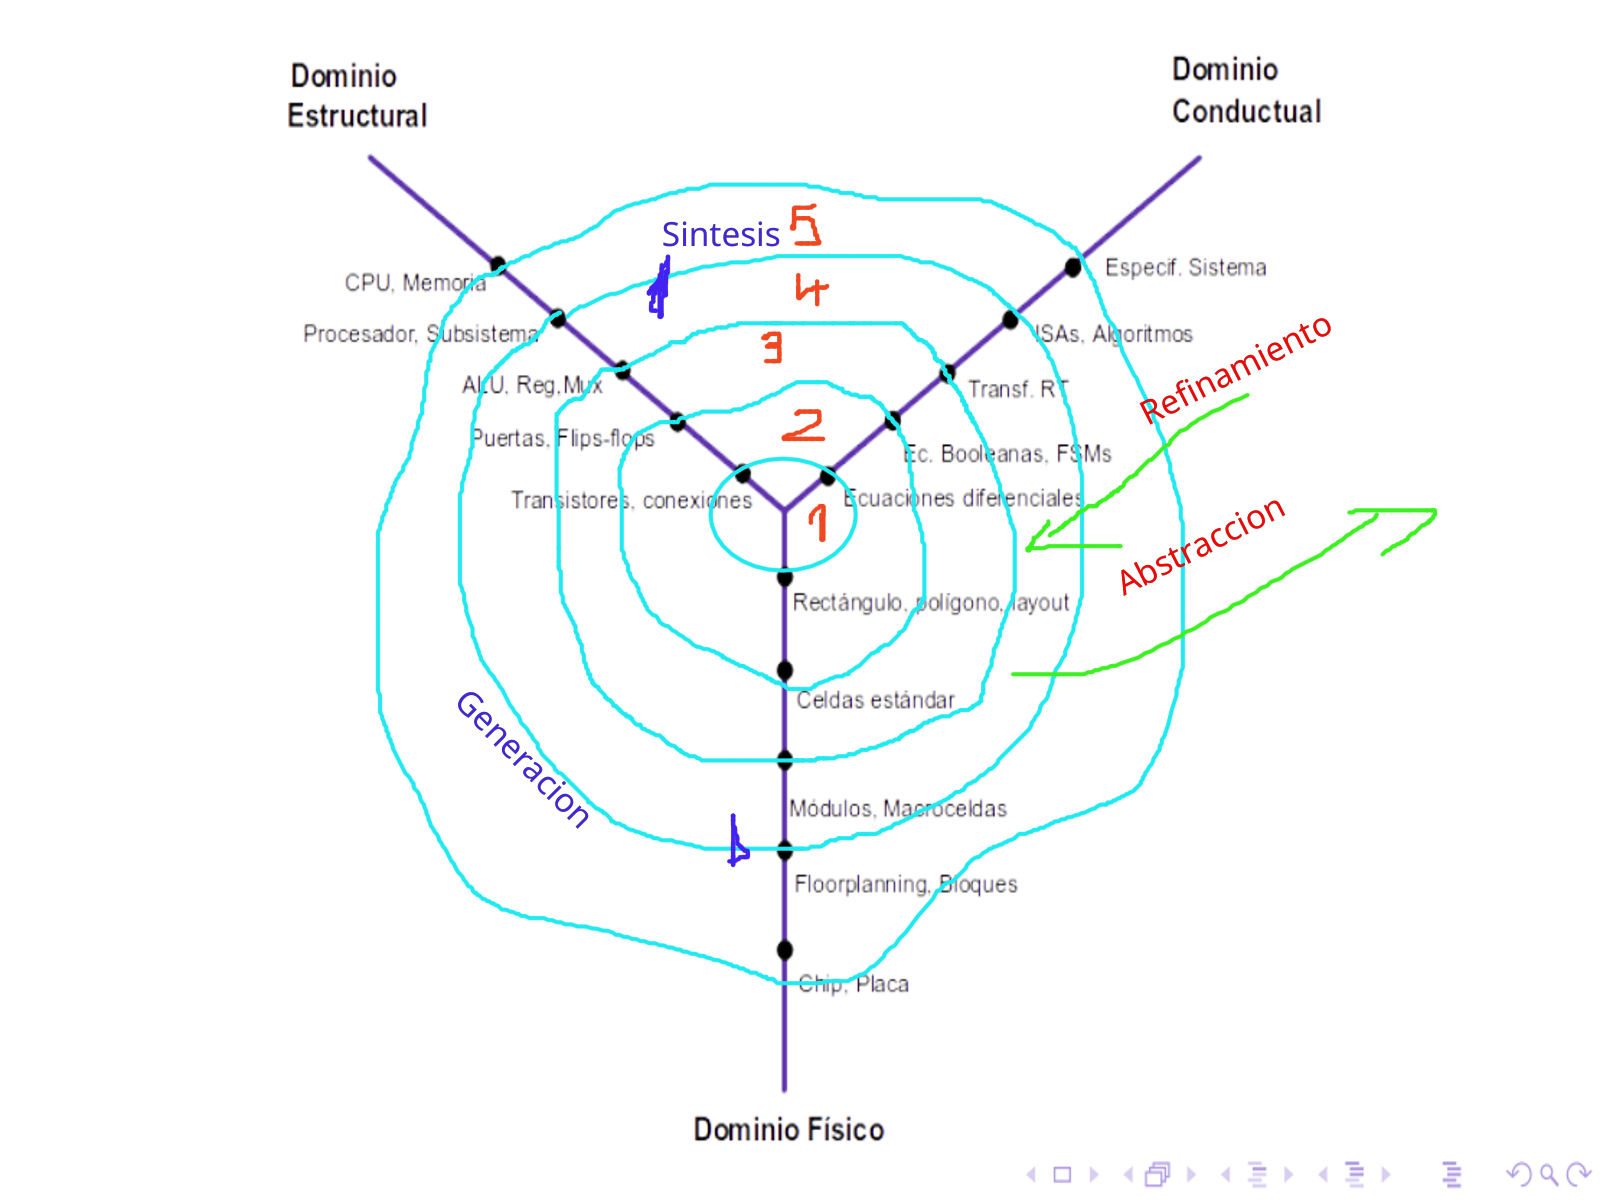
\includegraphics[width=1\textwidth]{figures/diagramaY.png}
\caption{Diagrama Y de Gajsky-Khun}
\label{diagramaY}
\end{figure}


\end{itemize}

\subsection{Nivel de abstracción}

\begin{itemize}
\item Circuito
Valores continuos, área de consumo.

\item Lógico
Falso o verdadero, computación, tiempo de conmutación, skew \footnote{Skew es }, área equivalente.

\item RT (Register Transfer)

Puertas equivalentes, control y procesamiento de tiempo discreto.

\item Algorítmico
Estructuras abstractas, dependencias, latencias, cadencia de datos, número de módulos.

\item Sistemas

Subsistemas, sincronización y protocolos, ancho de banda y MIPS \footnote{Microprocessor without Interlocked Pipeline Stages} 

\end{itemize}

Los niveles de abstracción se ilustran en la Figura \ref{diagramaY2}

\begin{figure}[H]
\centering
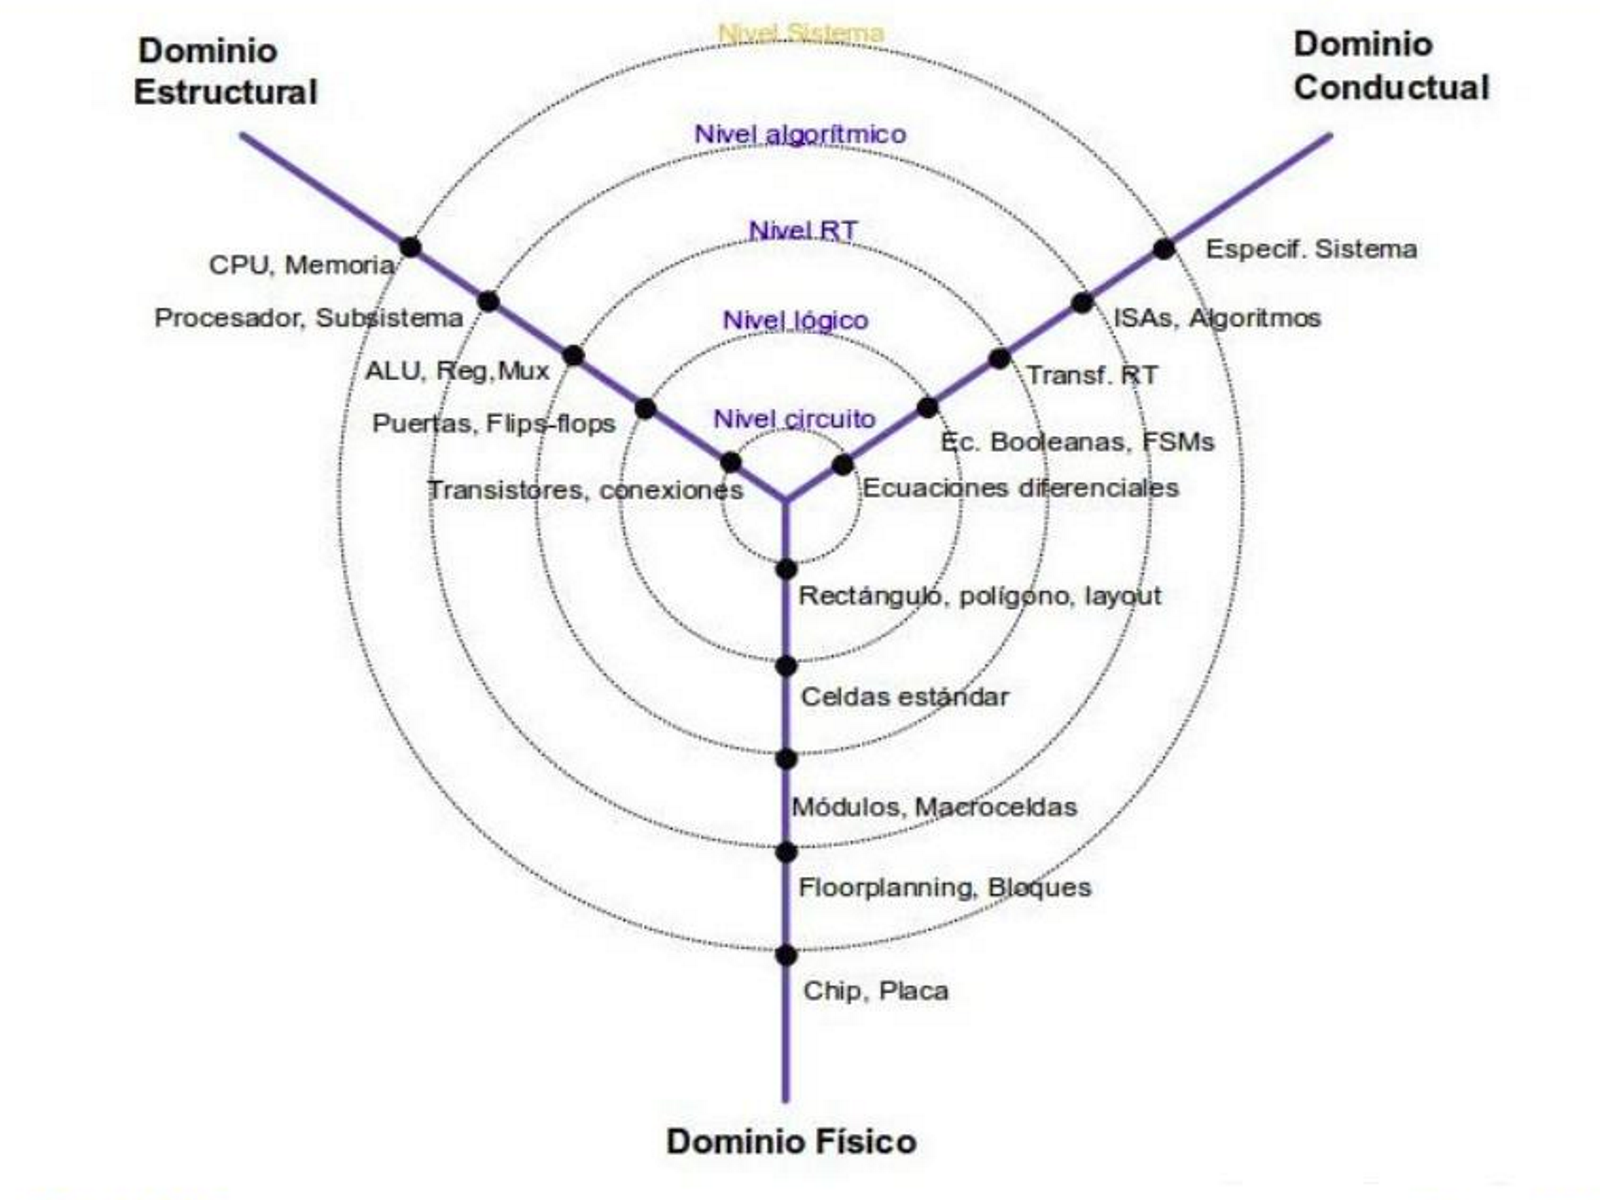
\includegraphics[width=1\textwidth]{figures/diagramaY2.png}
\caption{Niveles de proceso de abstracción según el  diagrama Y de Gajsky-Khun}\footnote{Gajsky-Khun es }
\label{diagramaY2}
\end{figure}
\section{Proceso de diseño}

Los dominios descriptivos se conmutan entre si y también hay un ciclo como se Ilustra en la Figura \ref{diagramaY3} 



\begin{figure}[H]
\centering
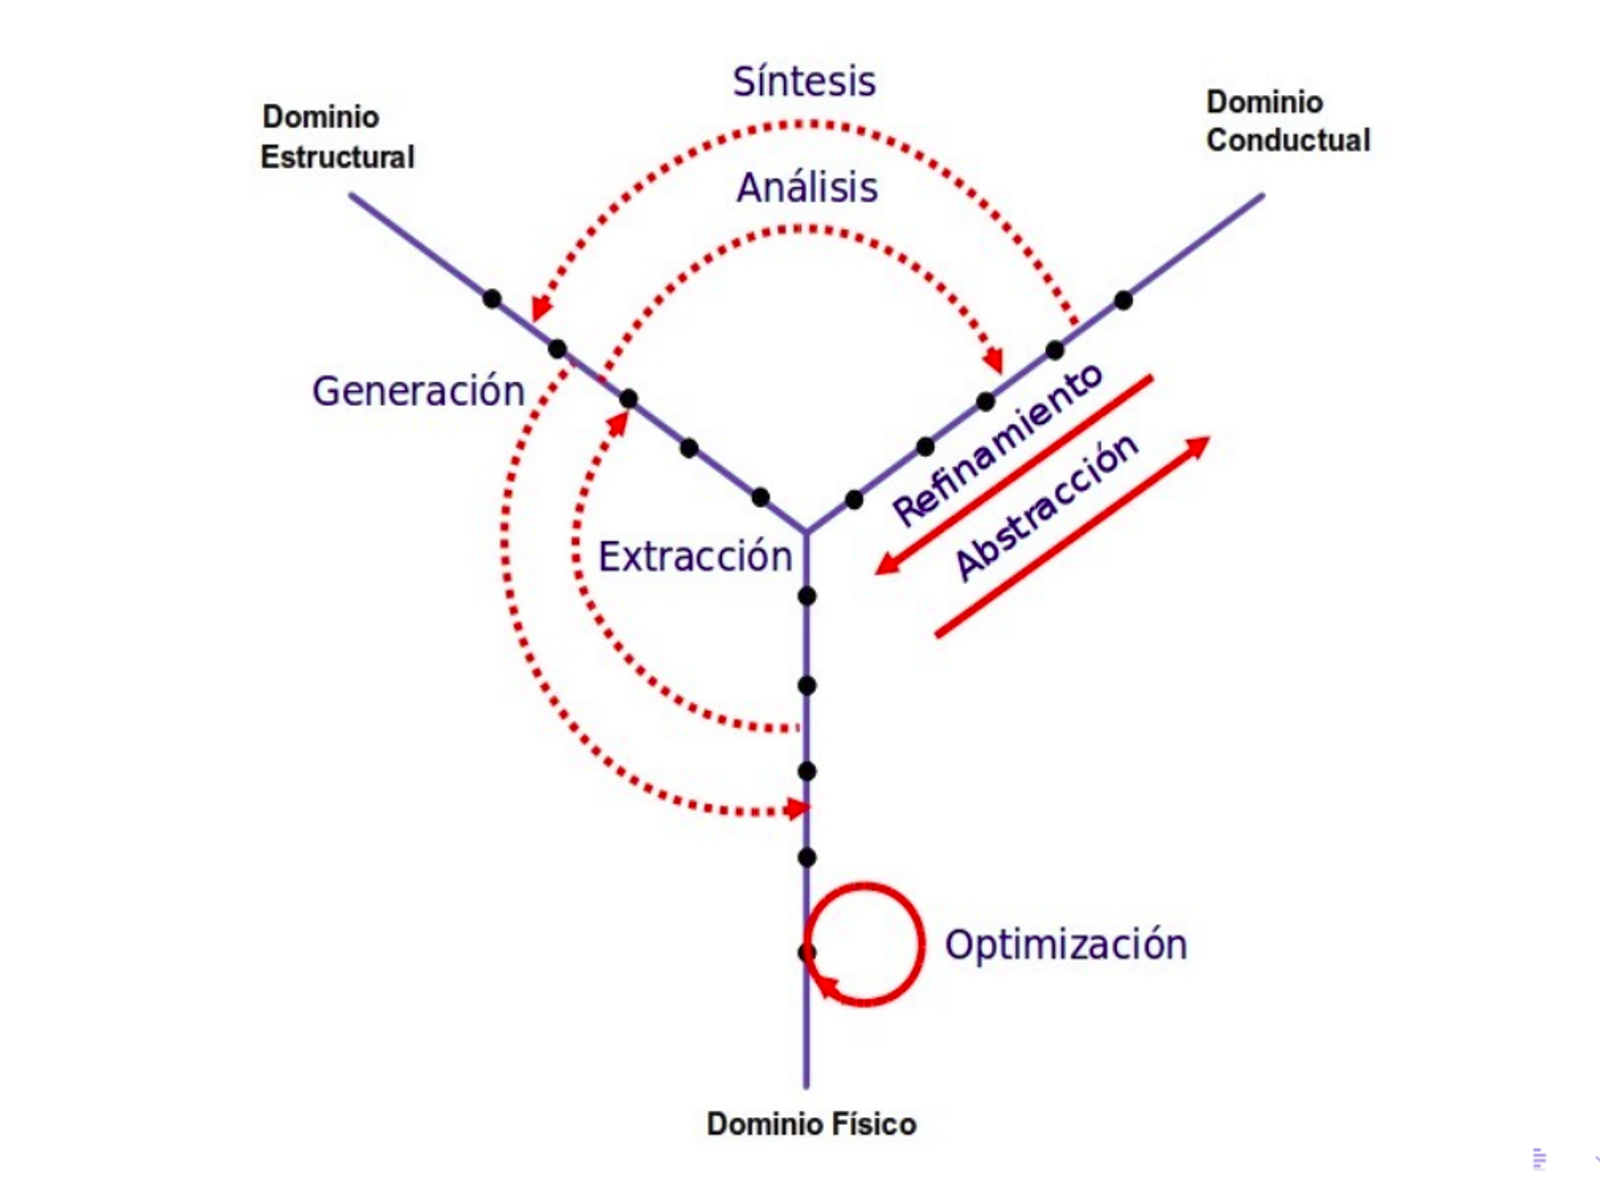
\includegraphics[width=1\linewidth]{figures/diagramaY3.png}
\caption{Conmutación entre los distintos dominios}
\label{diagramaY3}
\end{figure}

\begin{exercise}[Reloj]

Representación en el dominio conductual, estructural y físico de un reloj despertador sencillo.\\
Especificación

\begin{multicols}{2}
\begin{itemize}
\item Visualización LCD
Muestra horas, minutos y segundos.
\item 5 Conmutadores\\
S1: ajuste de hora\\
S2: ajuste de alarma\\
S3: avance de minutos\\
S4: avance de horas\\
 S5: Conexión de alarma\\
 

\textbf{ Modo de operación}
\item S1 está activo, se habilita S3 y S4 todo se observa en la LCD.
\item S2 está activo, se ajusta la hora con S3 y S4. En la LCD se muestran los cambios.
\item S5 está activo, la alarma se activa. Se producirá un sonido cuando las configuraciones y la alarma coincidan.

\end{itemize}


\begin{figure}[H]
\centering
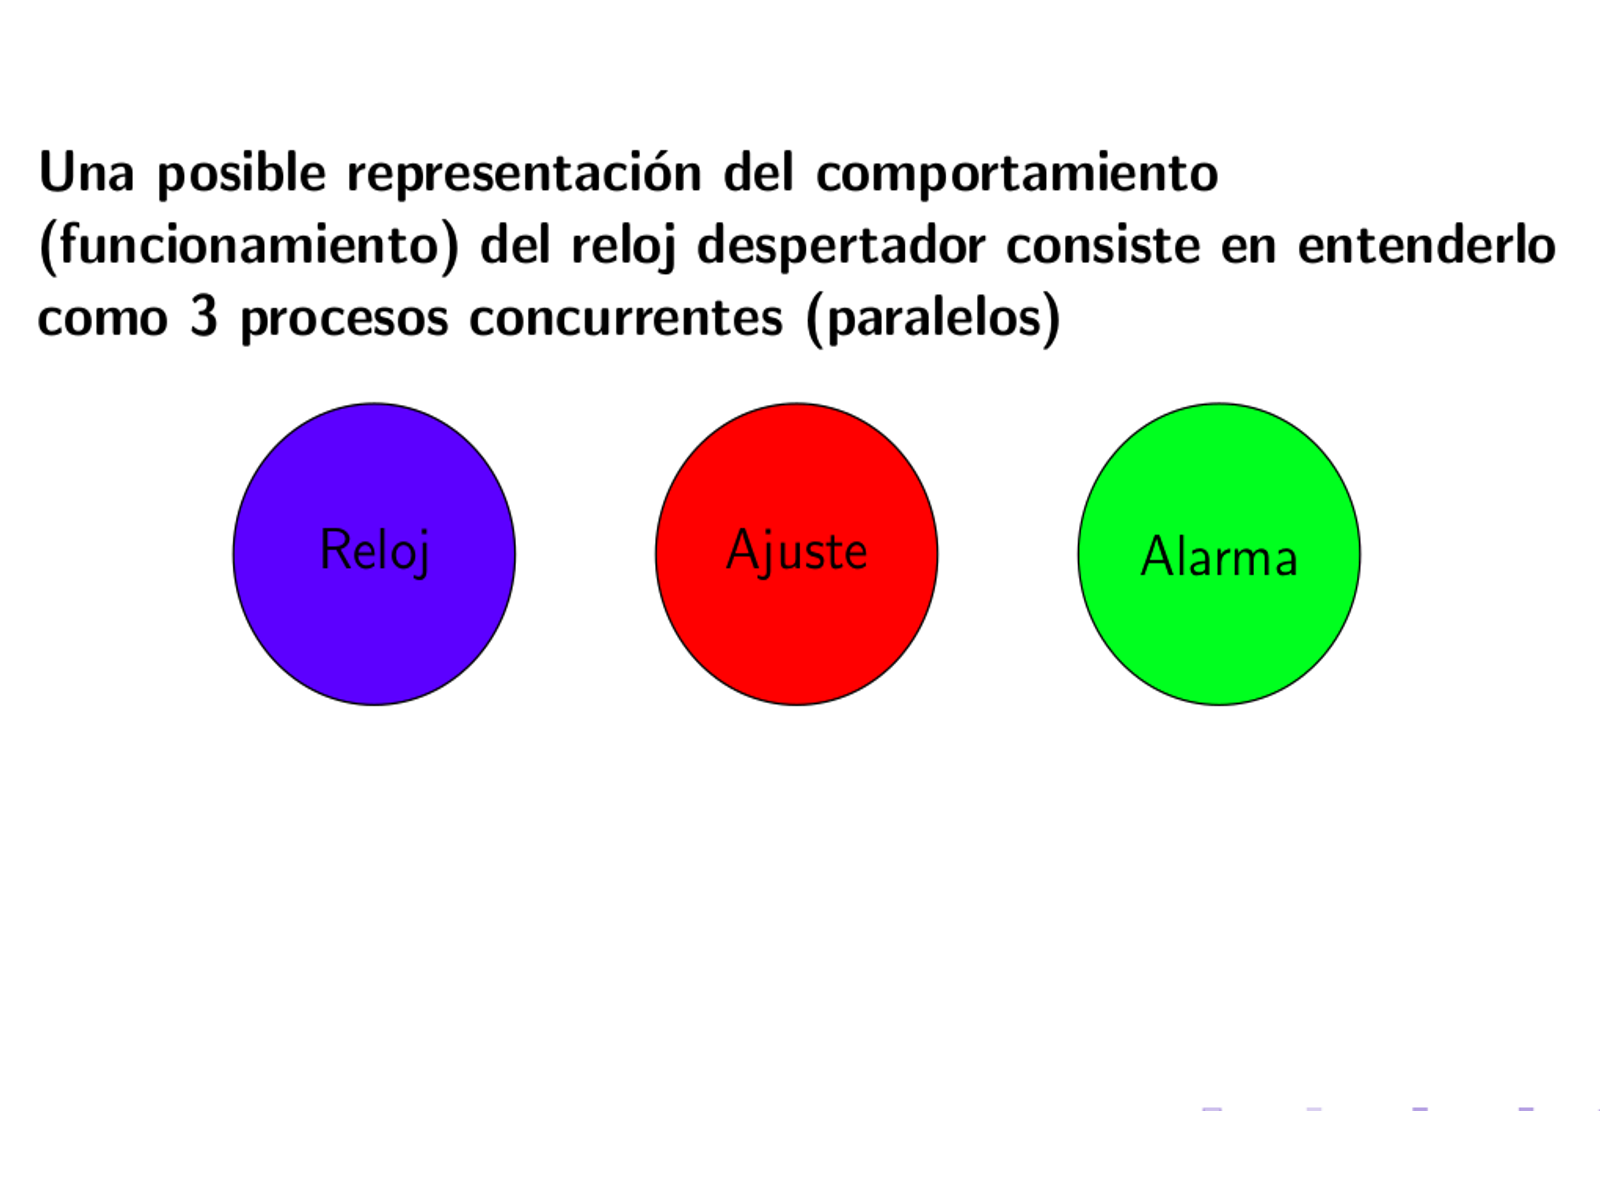
\includegraphics[width=1\linewidth]{figures/repFun1.png}
\caption{Funcionamiento en paralelo}
\label{repFun1}
\end{figure}
\vspace{0.2cm}

Respecto a la Figura \ref{repFun2}, en primera instancia si se detecta que la señal de pulso, que puede ser una onda cuadrada, es distinta de un valor referencia la variable Seconds aumenta; en caso contrario vuelve y pregunta si se detecta la "subida" de un pulso. Ahora, supóngase que Seconds es diferente de cero, entonces la función vuelve a ejecutarse desde el principio. En caso que todos los casos se den, el diagrama de flujo sigue sin hasta la última etapa que es la de horas, en este punto, se retorna al inicio.  

\begin{figure}[H]
\centering
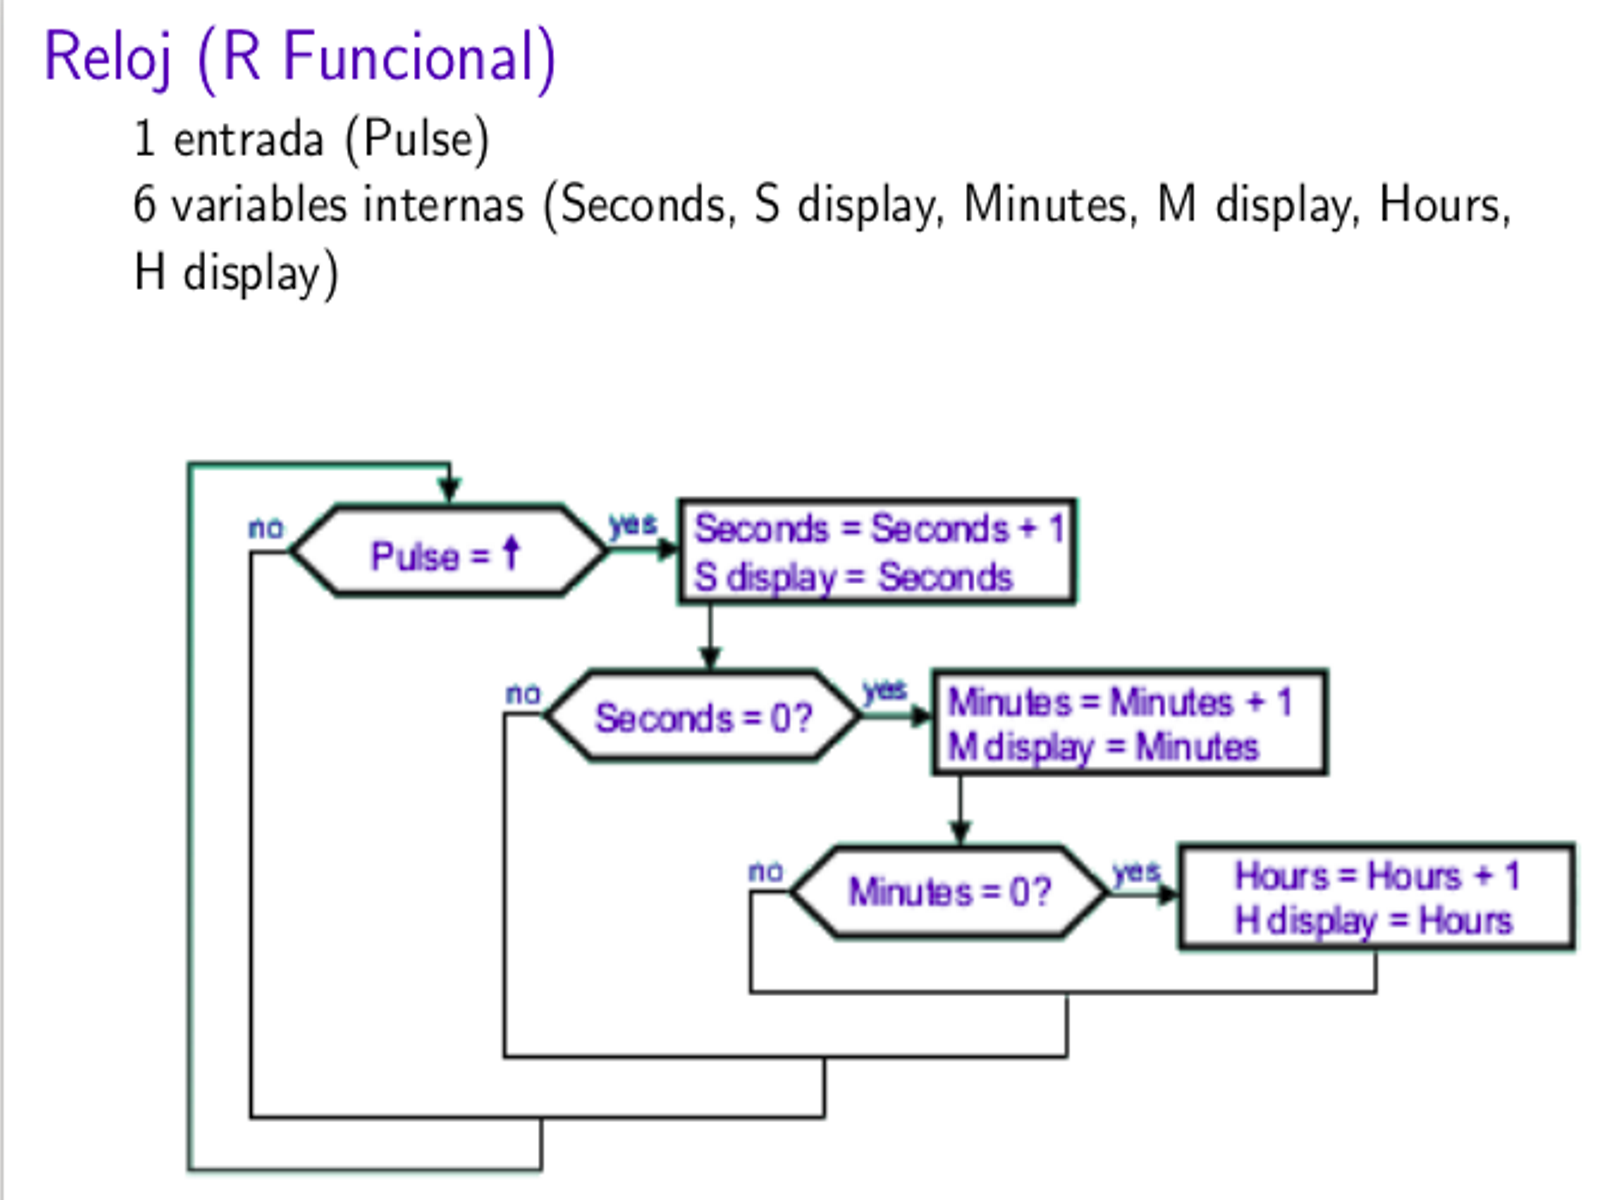
\includegraphics[width=1\linewidth]{figures/repFun2.png}
\caption{Representación funcional del reloj}
\label{repFun2}
\end{figure}
\vspace{0.2cm}

¿Cómo es posible que la variable Seconds sea cero si siempre aumenta? Es porque le puedo asignar por ejemplo 6 bits a la variable Seconds, lo que me indica que puedo almacenar hasta $63_{10}$. Cuando por ejemplo llego hasta el $111111_{2}$ y le aumento $1_{10}$ obtengo $1000000_2$, por tanto, se me desborda y solo el computador va a observar $000000_2$ porque tengo 6 bits.\\

Paso a seguir es el diagrama funcional de ajuste en horas y la alarma que se ilustra en la Figura \ref{repFun3}. Sin embargo, surge un inconveniente, ¿Cómo se hace cuando S1 y S2 se oprimen al tiempo?. En esta instancia, es posible que esto suceda y como se verá más adelante para no emplear más componentes se puede solucionar en la descripción física. 

 
\begin{figure}[H]
\centering
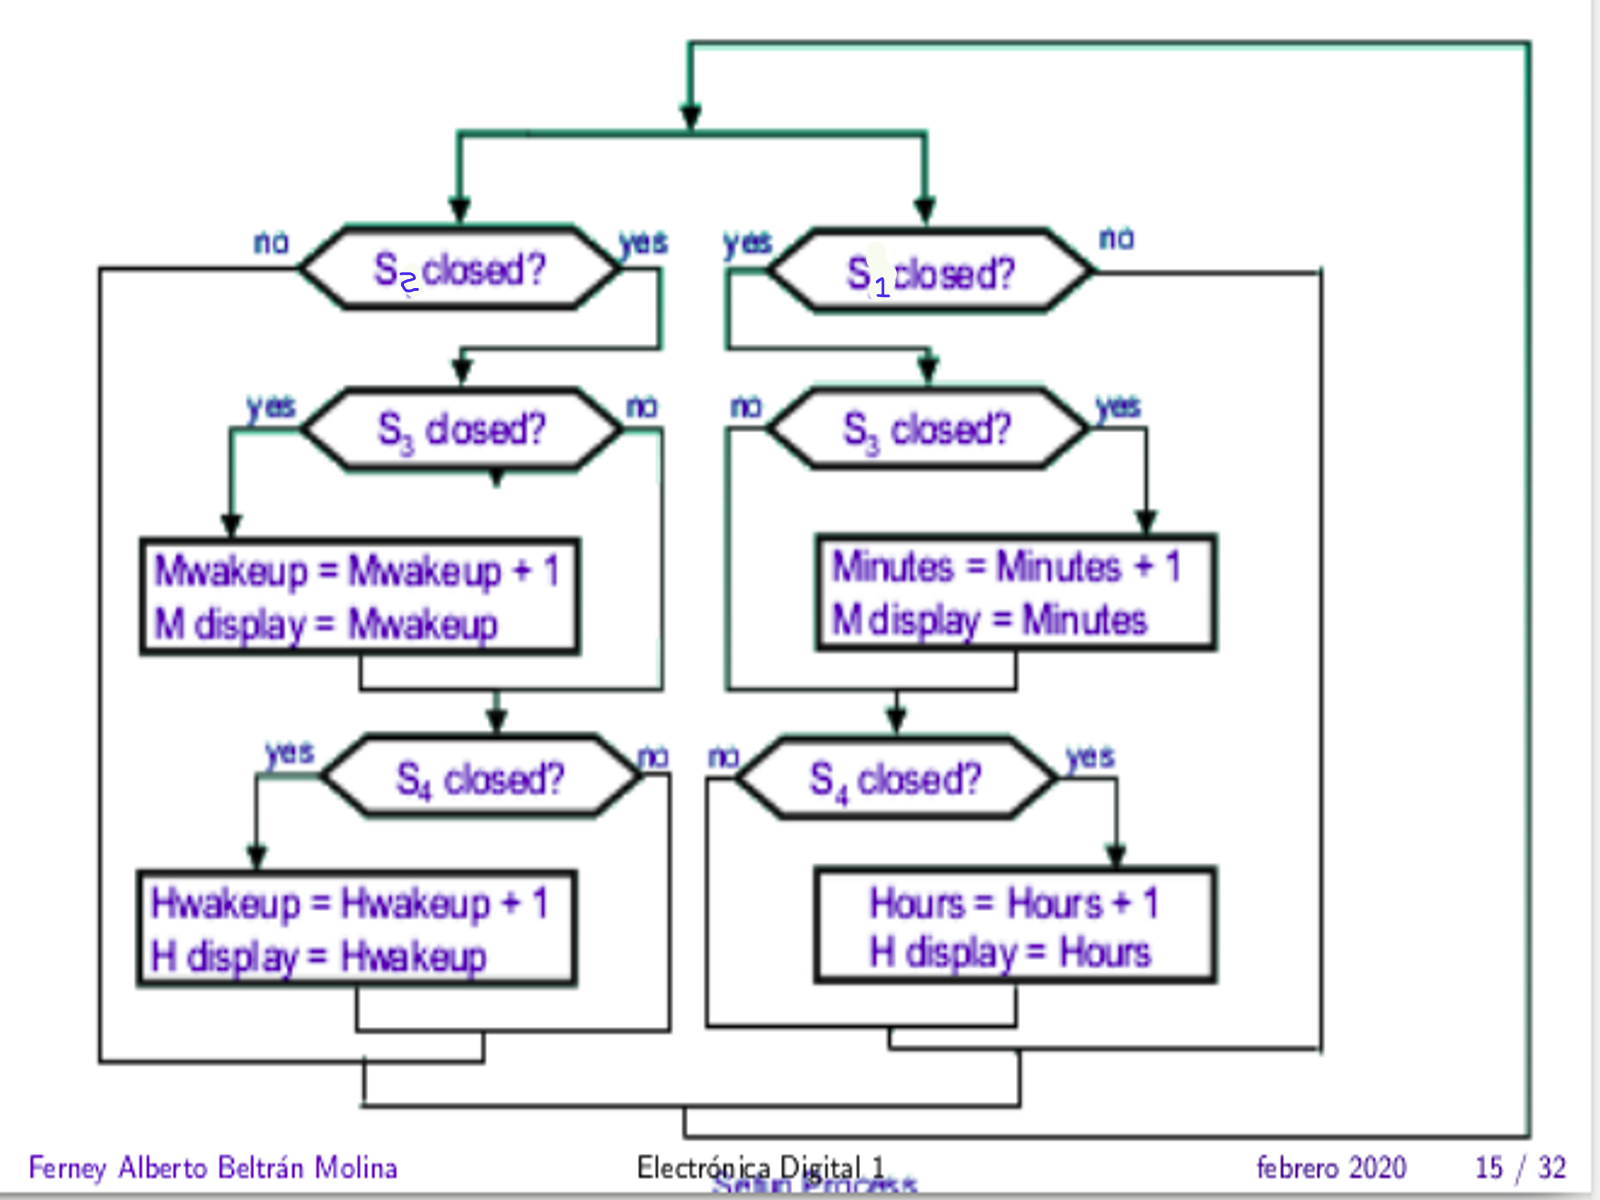
\includegraphics[width=1\linewidth]{figures/repFun3.png}
\caption{Diagrama funcional del ajuste}
\label{repFun3}
\end{figure}
\vspace{0.2cm}

Por último, se hace la descripción física de la alarma en la Figura \ref{repFun4}. 

\begin{figure}[H]
\centering
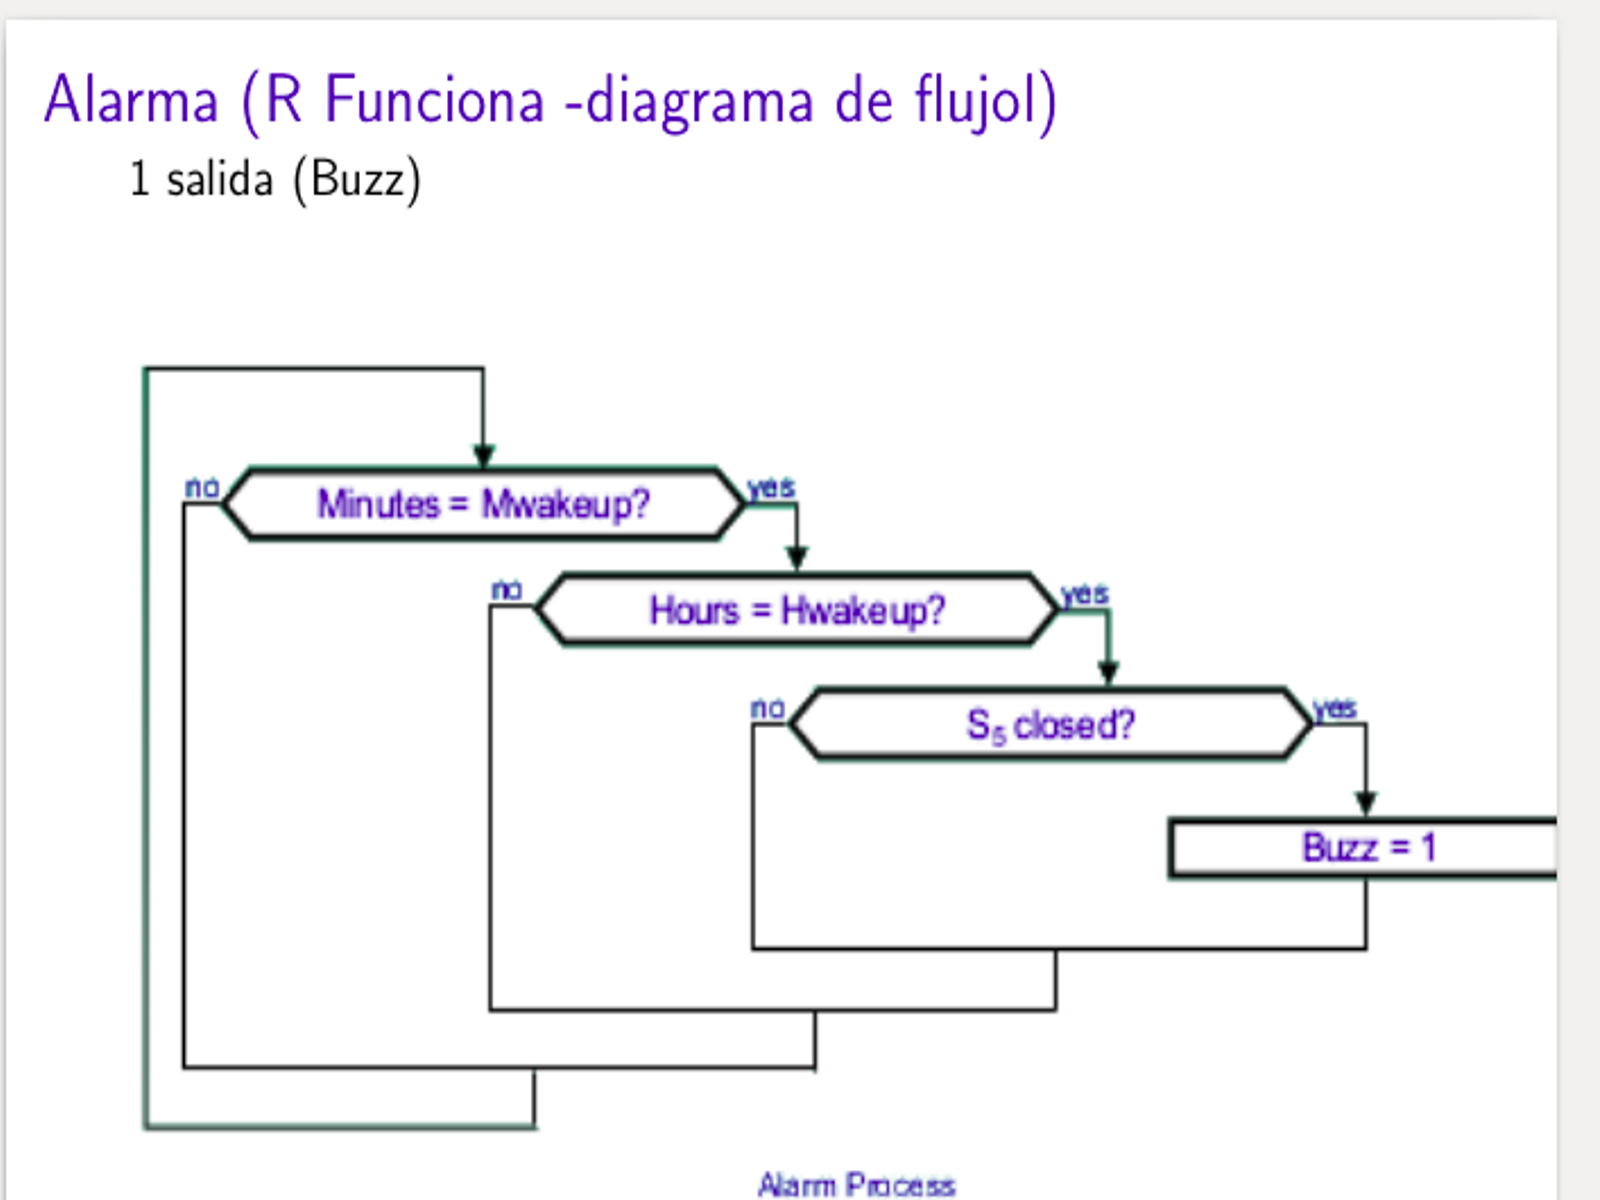
\includegraphics[width=1\linewidth]{figures/repFun4.png}
\caption{Diagrama de flujo de la la alarma}
\label{repFun4}
\end{figure}
\vspace{0.2cm}

En la Figura \ref{repEst1} está la representación estructural. Se puede observar que si se oprime S1 Y S2 al mismo tiempo, se va a mostrar en la LCD los datos del reloj y si se procede a configurar la hora del reloj, también se cambia la de la alarma ¿Cómo se soluciona para que no pase esto? la representación física da una solución astuta. 

\begin{figure}[H]
\centering
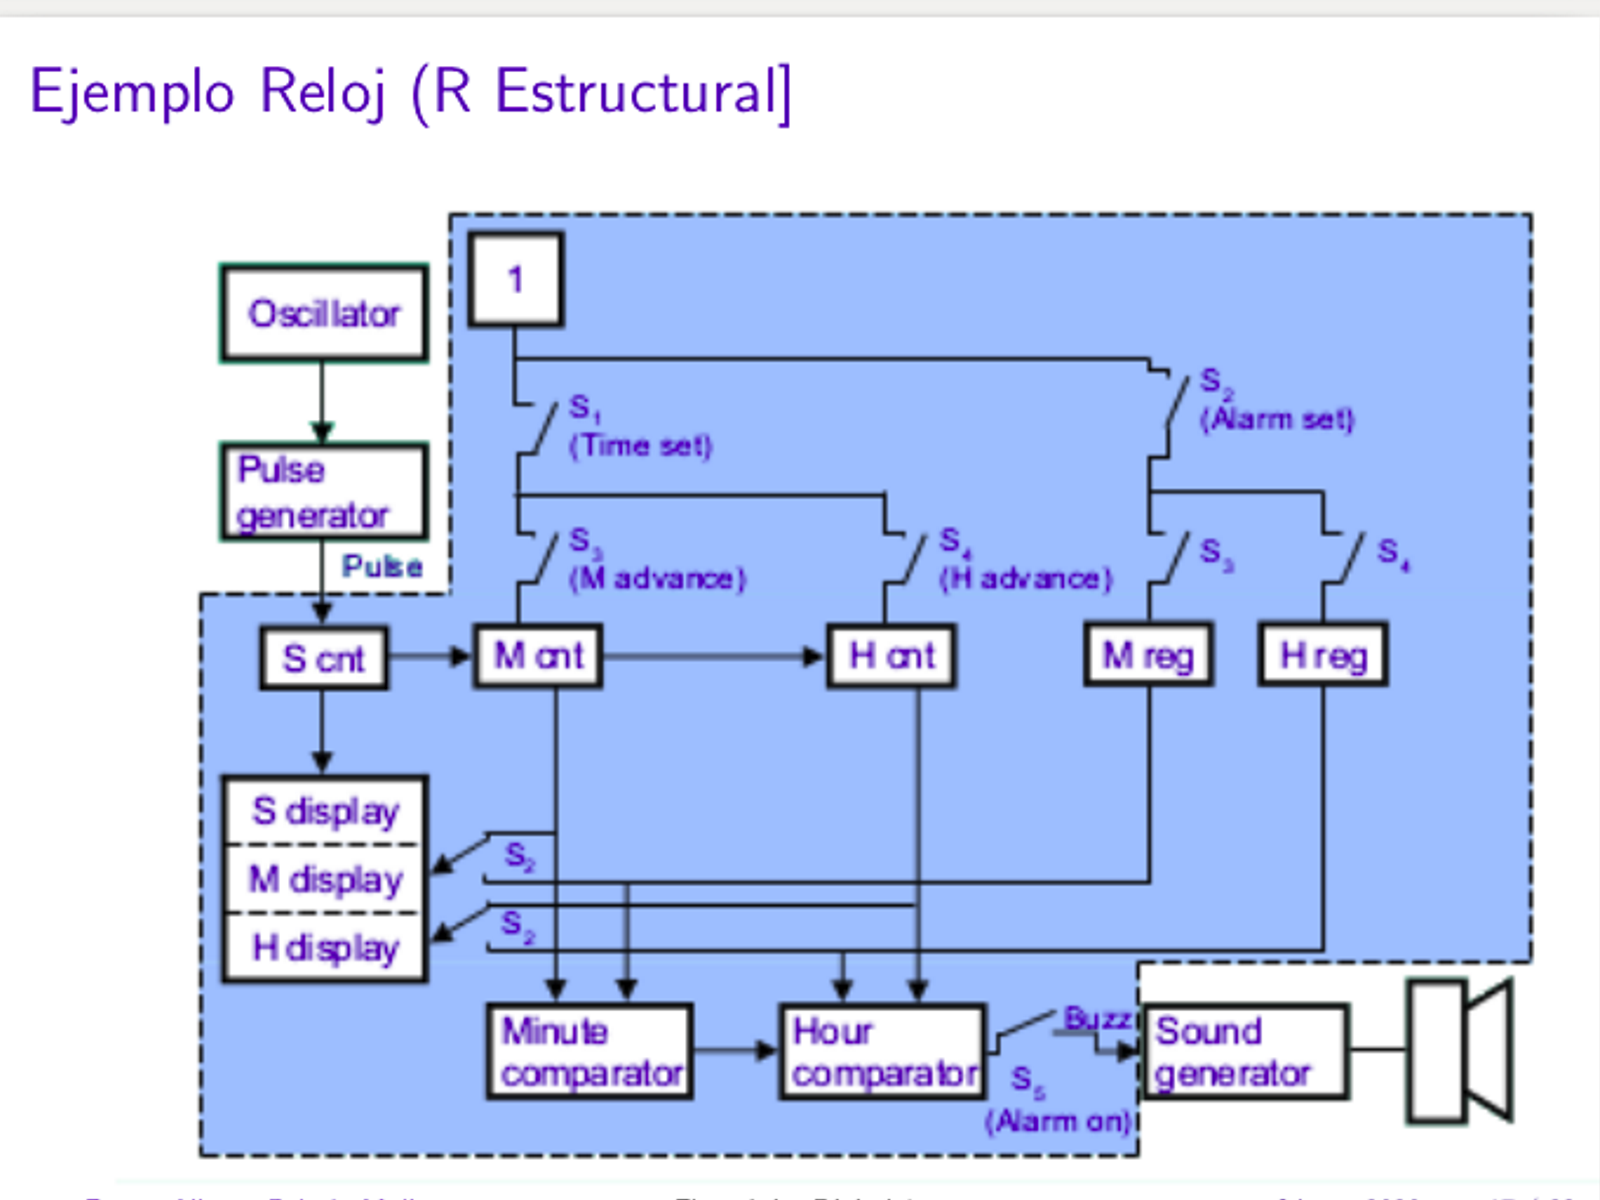
\includegraphics[width=1\linewidth]{figures/repEst1.png}
\caption{Representación estructural del reloj}
\label{repEst1}
\end{figure}
\vspace{0.2cm}

En la Figura \ref{repFis1} se hace la representación física que permite solucionar el problema de oprimir a S1 y S2. Como se puede observar, solo se puede estar en una configuración a la vez. 

\begin{figure}[H]
\centering
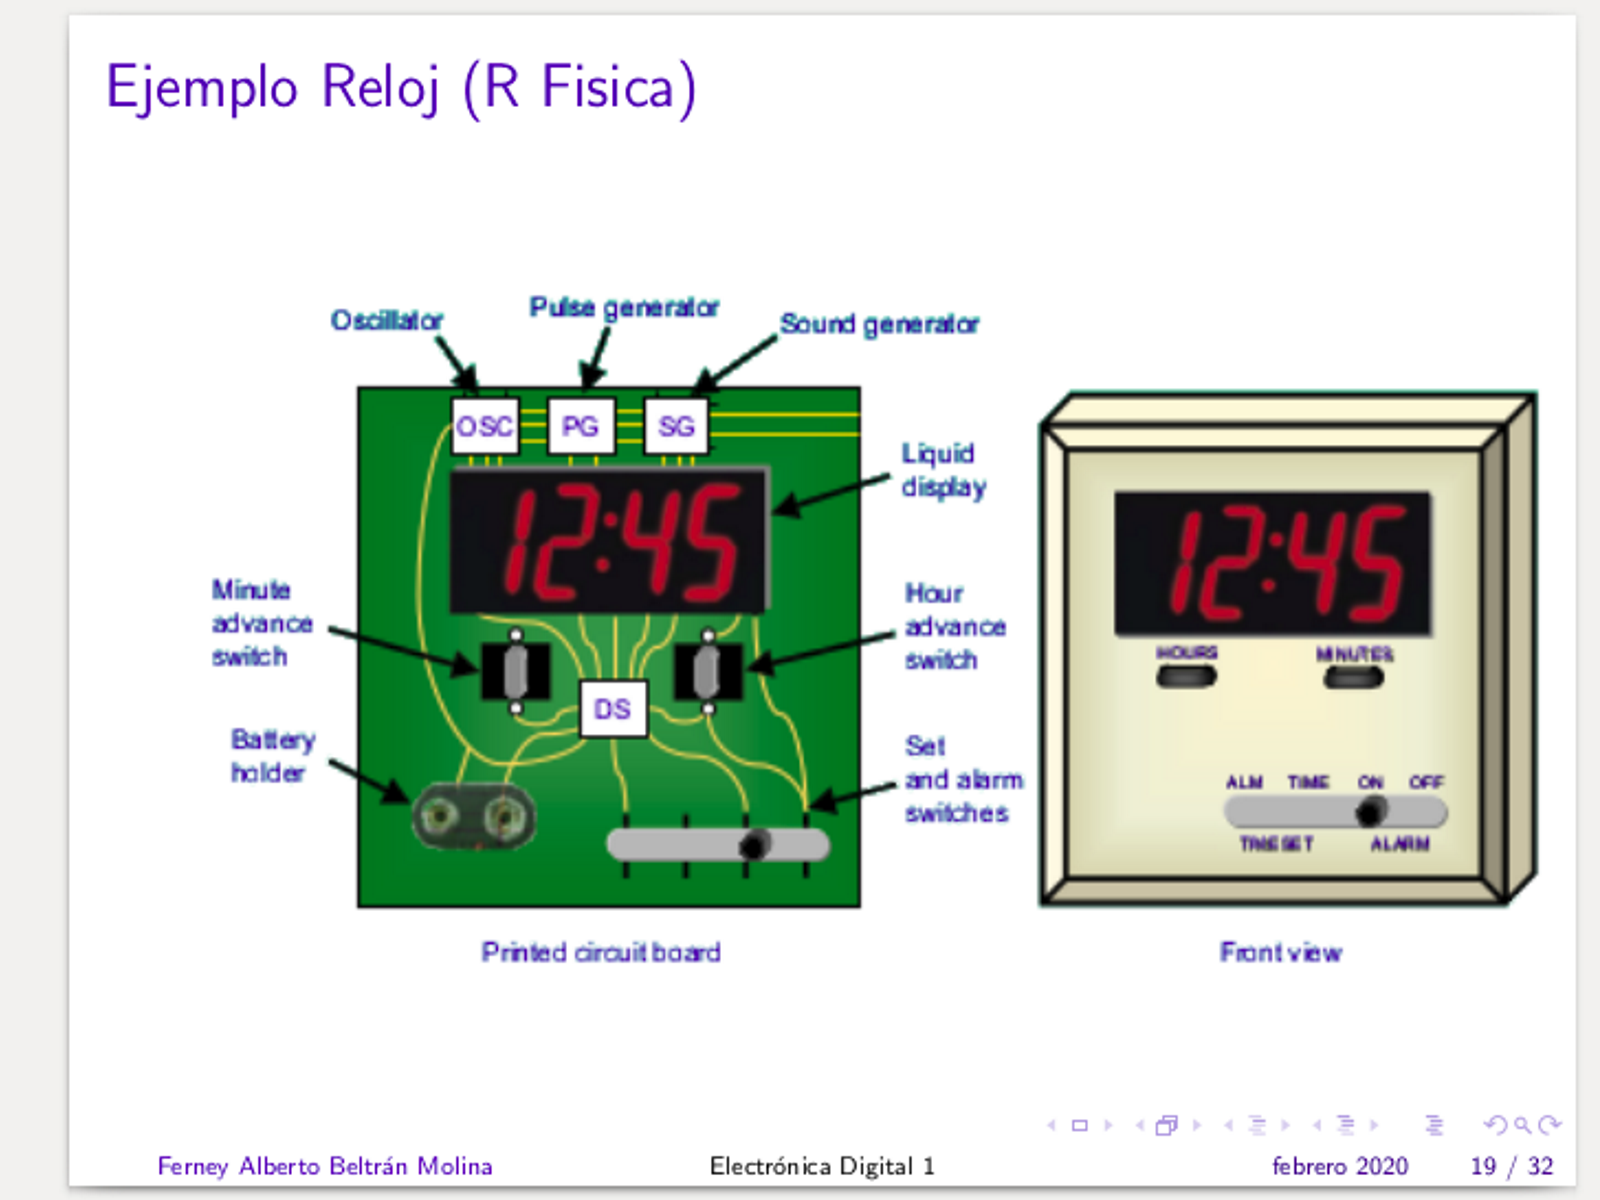
\includegraphics[width=1\linewidth]{figures/repFis1.png}
\caption{Representación física del reloj}
\label{repFis1}
\end{figure}
\vspace{0.2cm}
\end{multicols}
\end{exercise}

\section{Proceso de diseño}


\section{Resumen} 
\section{Ejercicios} 

\begin{exercise}[Cerradura con Llave]

Diseñar una cerradura digital que le ingresa un número de tres dígitos.

\begin{enumerate}
\item Si hay un error en cualquier dígito se debe bloquear la puerta.
\item Dos entradas: Reset y bus de datos con números.
\item Una salida: Cerradura abierta o cerrada.
\item Memoria: almacena la clave para poderse comparar.

\end{enumerate} 


\end{exercise}

\chapter{Semana 2}

\section{Tipos de sistemas de numeración}
\begin{enumerate}
\item Sistema Hexadecimal
Tiene 16  símbolos, empezando desde 0.
\item Sistema Decimal
Tiene 10 símbolos, empezando desde 0.
\item Sistema Octal
Tiene 8, empezando desde 0.
\item Sistema Binario
Tiene 2, empezando desde 0.

En la Tabla \ref{sistemas}, se observan los distintos sistemas y sus símbolos.
\end{enumerate}

                                 
\begin{table}[H]
        \caption{}
        \label{sistemas}
        \begin{center}
        \begin{tabular}{|c||c||c||c|}
        \hline
        \multicolumn{4}{|c|}{Sistemas} \\ \hline    
        
        Hexadecimal&Decimal &Octal &Binario \\ \hline        
		        1&1&1&1\\ \hline
		        2&2&2&10\\ \hline
		        3&3&3&11\\ \hline
		        4&4&4&100\\ \hline
		        5&5&5&101\\ \hline
		        6&6&6&110\\ \hline
		        7&7&7&111\\ \hline
		        8&8&10&1000\\ \hline
		        9&9&11&1001\\ \hline
		        A&10&12&1010\\ \hline
		        B&11&13&1011\\ \hline
		        C&12&14&1100\\ \hline
		        D&13&15&1101\\ \hline
		        E&14&16&1110\\ \hline
		        F&15&17&1111\\ \hline
		        
        
        \end{tabular}
        \end{center}
    \end{table}
    \vspace{0.2 cm}
    
   \subsection{Conversiones}
   -En el sistema base 16, cada dígito se representa con 4 bits.\\
   -Se puede dividir sistema binario en 4 bits de derecha a izquierda, luego, se hace la equivalencia a hexadecimal.
   -Se puede dividir sistema binario en 3 bits de derecha a izquierda, luego, se hace la equivalencia a octal
   
   
    \subsection{Sistemas binarios puros}
    
    \begin{itemize}
    \item Sólo números positivos.
    \item Para n bit, representa $2^n$ representaciones distintas.
    \item La representación va desde 0-($2^n-1$).
    \end{itemize}
   
   \subsection{Operaciones en el sistema binario}

\begin{multicols}{2}
Suma

\begin{itemize}
\item $0+0=0$
\item $0+1=1$
\item $1+0=1$
\item $1+1=1$ \textbf{0} llevo \textbf{1}

\end{itemize}

Resta

\begin{itemize}
\item $0-0=0$
\item $0-1=1$ \textbf{1} presta \textbf{1}
\item $1-0=1$
\item $1-1=0$ 

\end{itemize}
\end{multicols}   
   
  \section{Complemento de un número}
  
   \section{Ejercicios}
   \section{Resumen}

\chapter{Semana 3}

\section{Introducción a la lógica combinacional}

En electrónica digital un circuito hace:
\begin{itemize}
\item Entradas y salidas discretas.
\item Especificar la función que relaciona entradas y salidas.
\item Especifica el tiempo de retardo de cada entrada y salida.
\end{itemize}

\subsection{Tipo de circuitos digitales}

\begin{itemize}
\item circuitos combinacionales\\

Sus valores de salida dependen únicamente de combinaciones de las entradas en un determinado tiempo.

\item circuitos secuenciales.\\

Dependen de valores almacenados y actuales, en otras palabras, depende de un secuencia de entrada.\\

\end{itemize}


La Figura \ref{cirDig} representa los tipos de circuitos.


\begin{figure}[H]
\centering
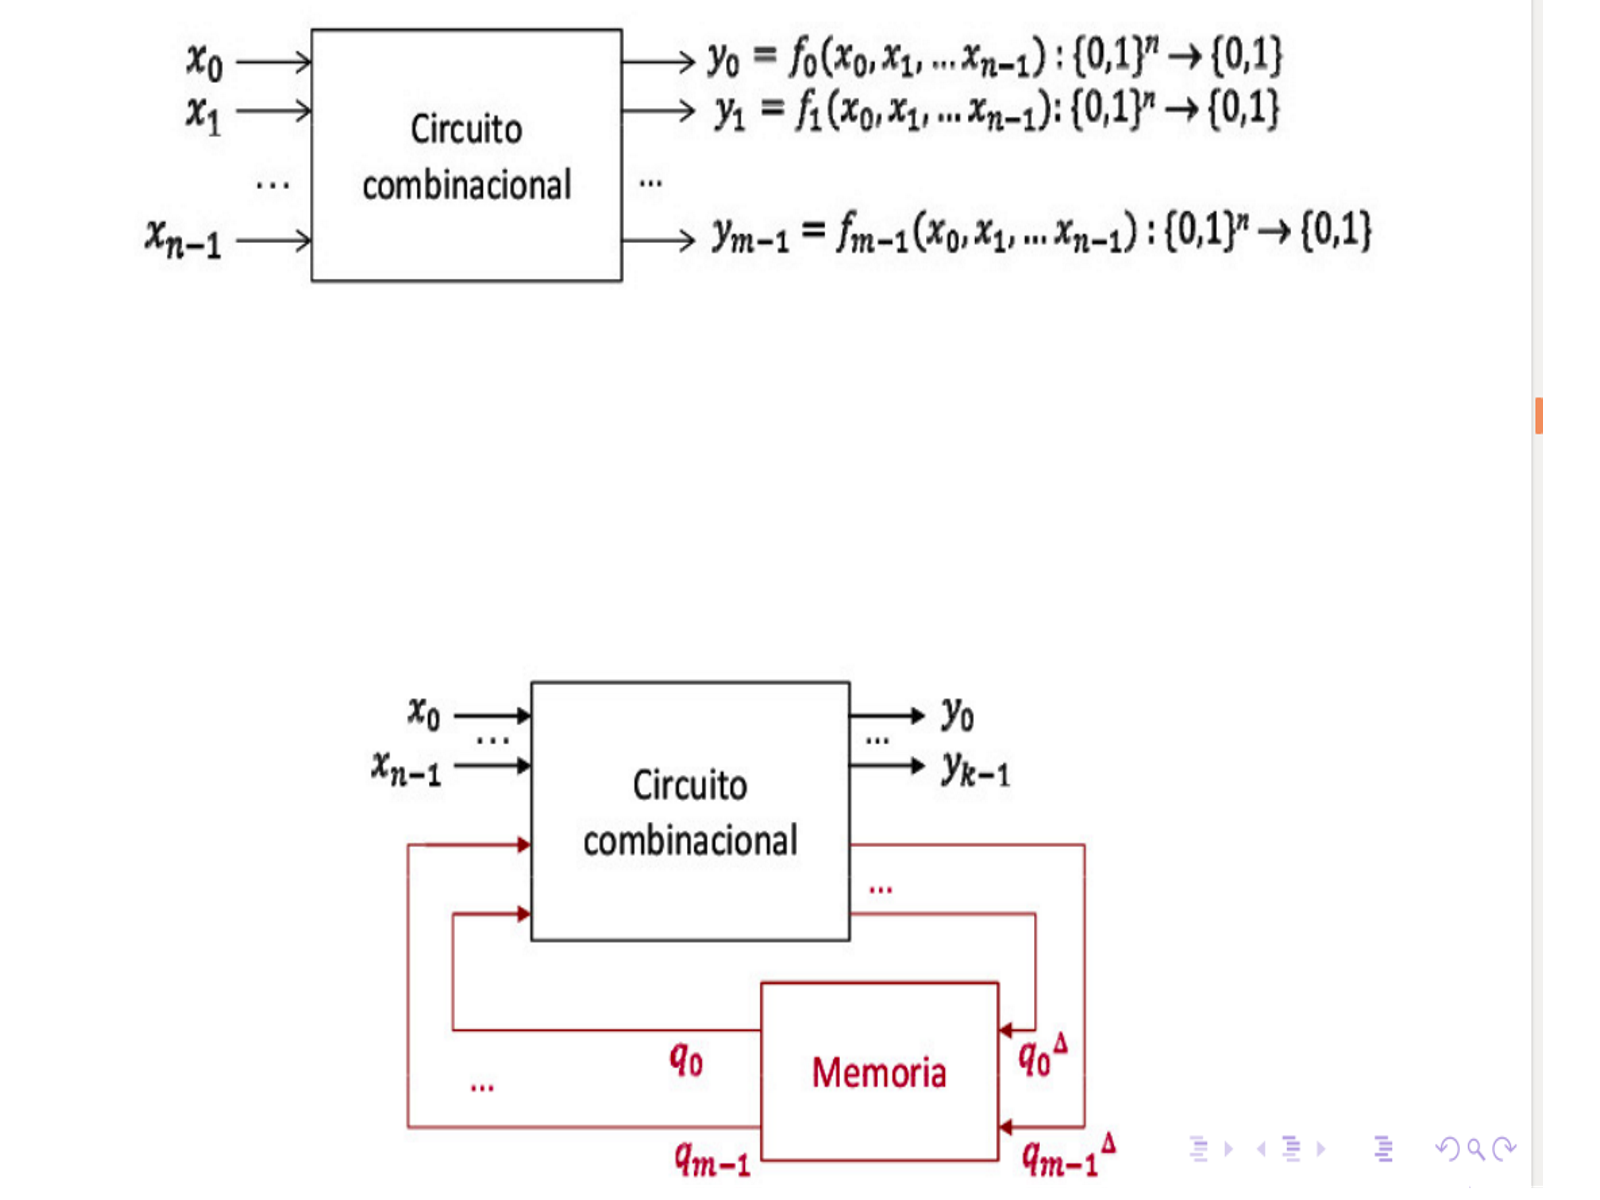
\includegraphics[width=1\linewidth]{figures/cirDig1.png}
\caption{Tipos de circuitos digitales}
\label{cirDig1}
\end{figure}
\vspace{0.2cm}

\begin{example}[Sumador de 4 bits]
\begin{multicols}{2}

La Figura \ref{ejeSum1} es un circuito secuencial, ya que depende de valores adicionales de la entrada. 

\begin{figure}[H]
\centering
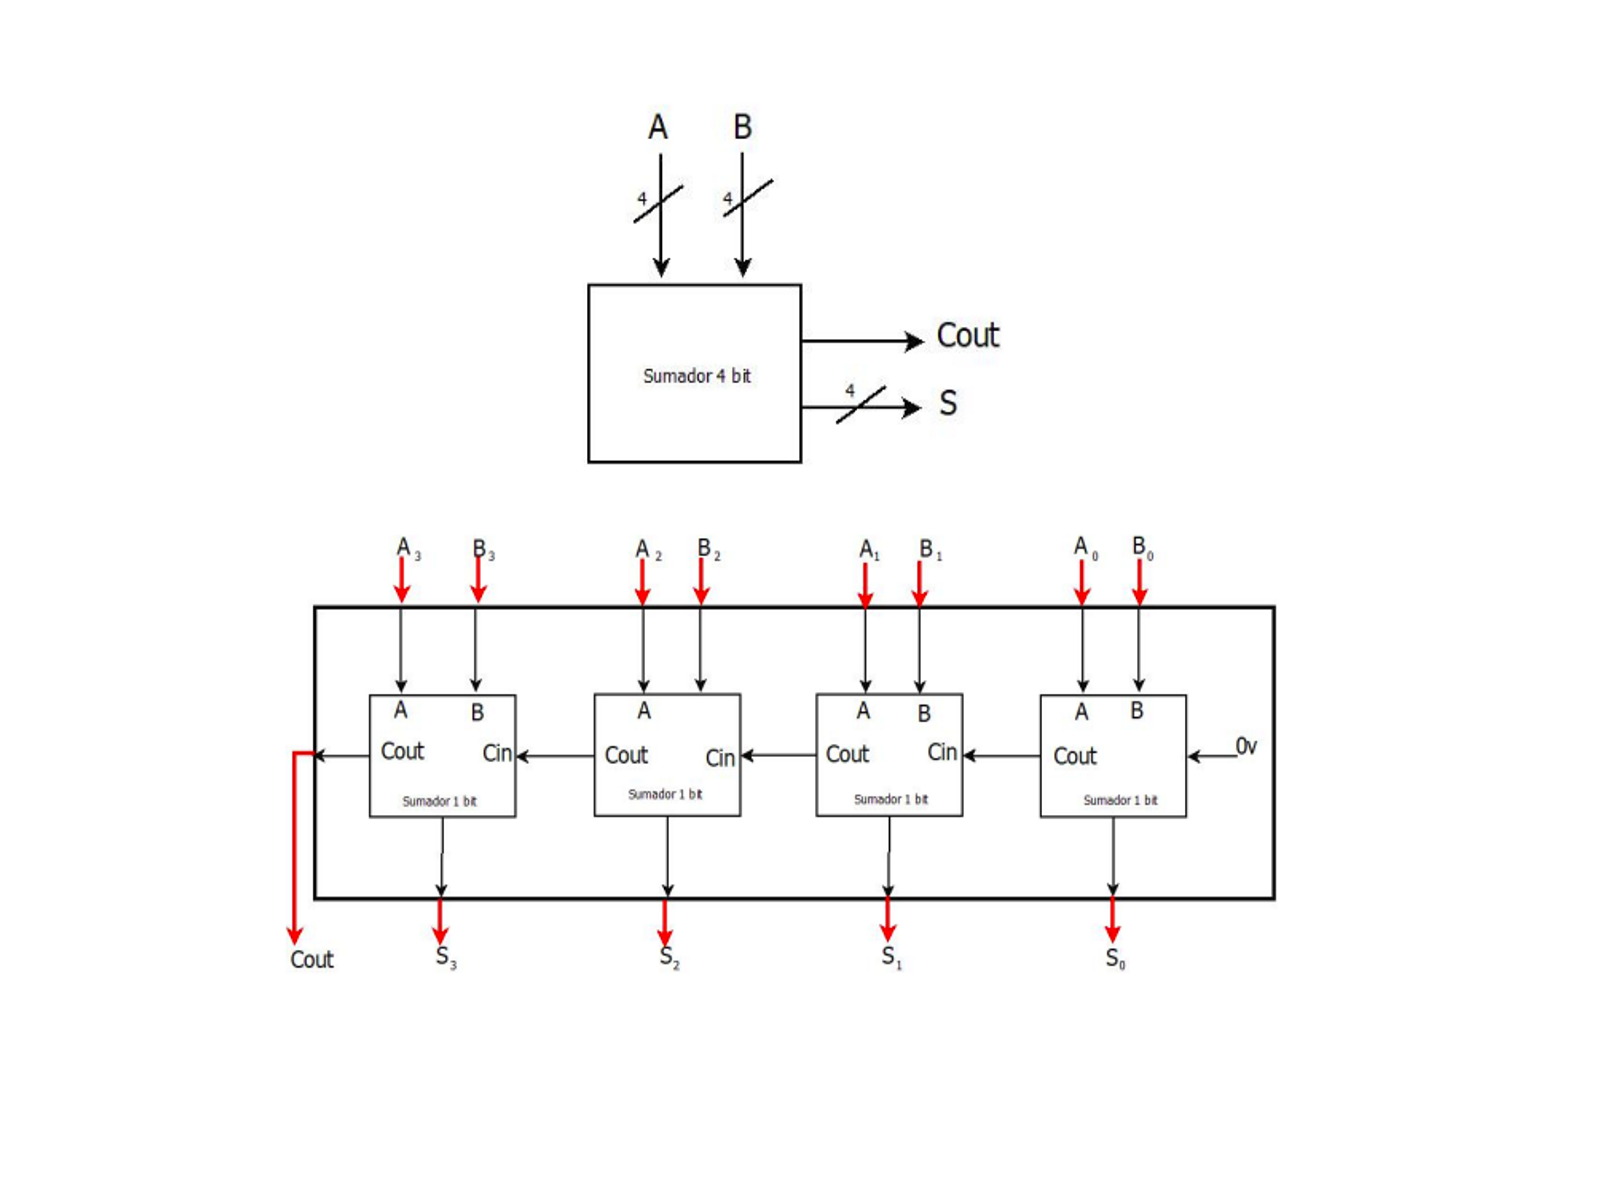
\includegraphics[width=1\linewidth]{figures/ejeSum1.png}
\caption{Sumador de 4 bits \cite{Beltran}}
\label{ejeSum1}
\end{figure}
\vspace{0.2cm}

En la  Figura \ref{ejeSum2} representa la manera de solucionar el circuito a partir de tablas de verdad.  

\begin{figure}[H]
\centering
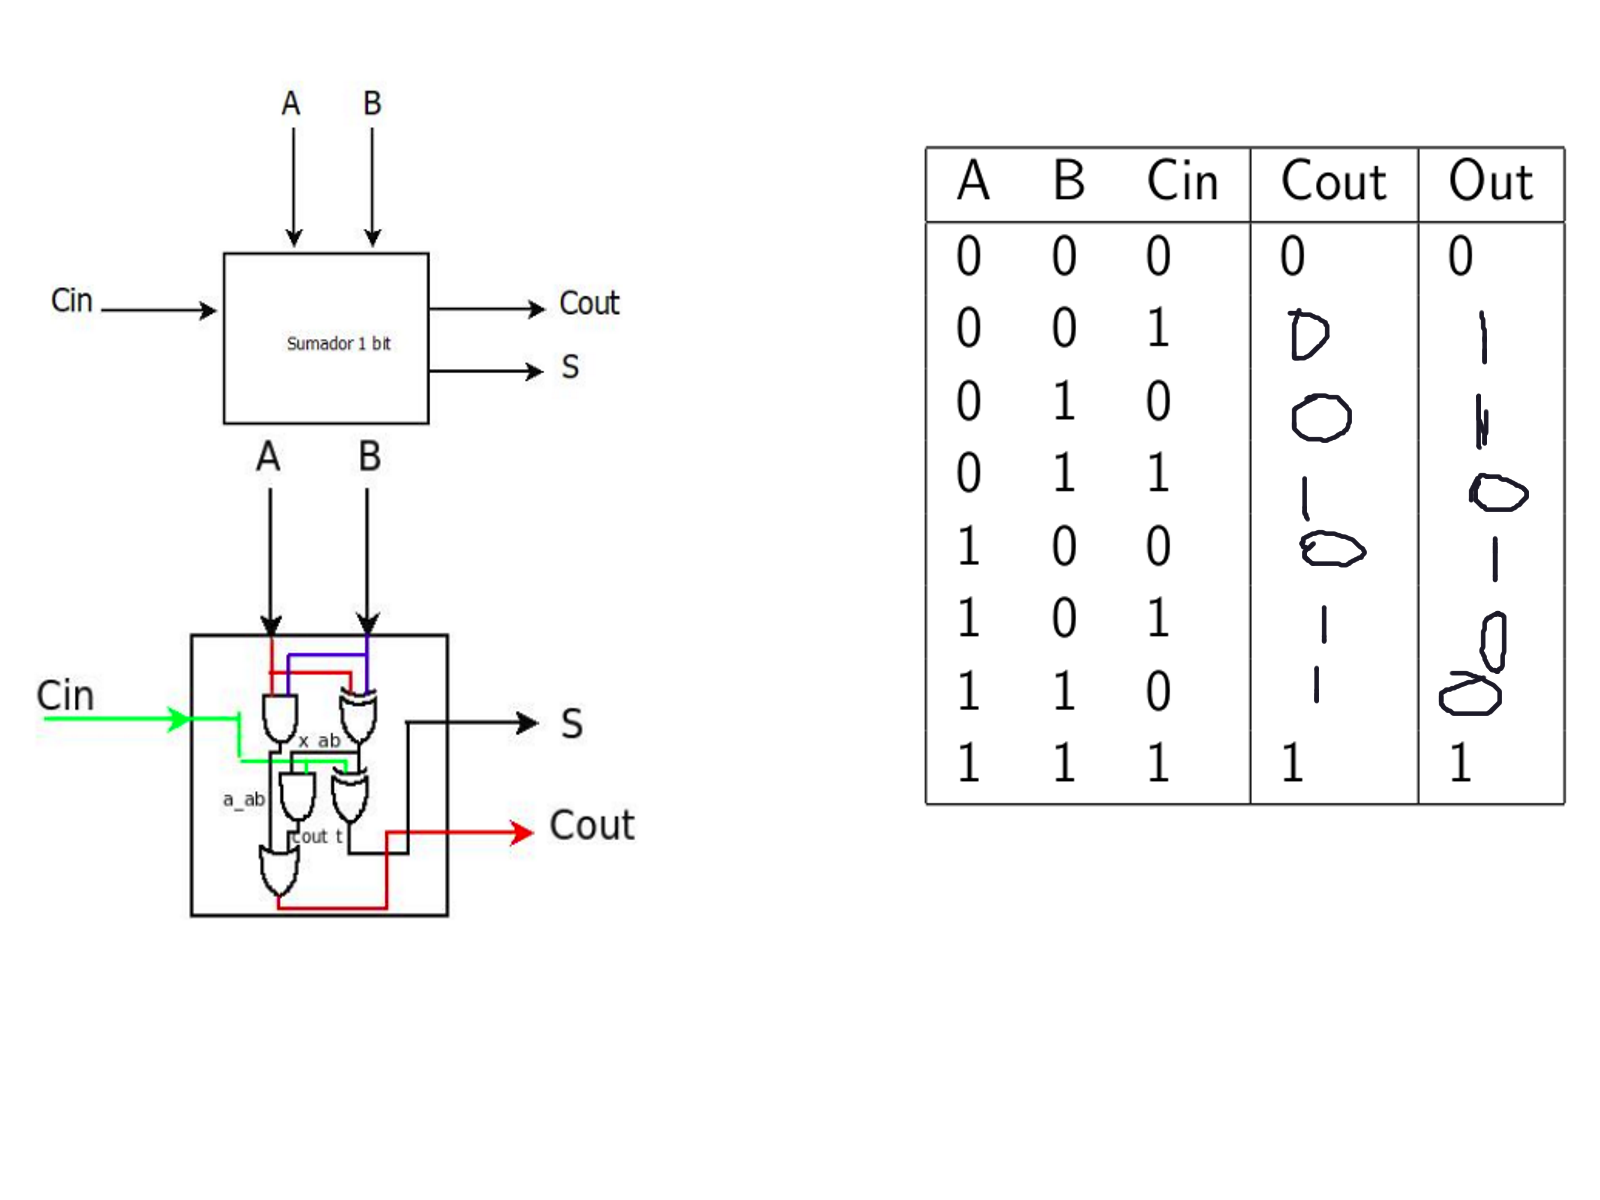
\includegraphics[width=1\linewidth]{figures/ejeSum2.png}
\caption{Sumador a partir de tablas de verdad}
\label{ejeSum2}
\end{figure}
\vspace{0.2cm}

En la Figura \ref{ejeSum3} muestra las compuertas lógicas NOT, AND, OR, XOR.

\begin{figure}[H]
\centering
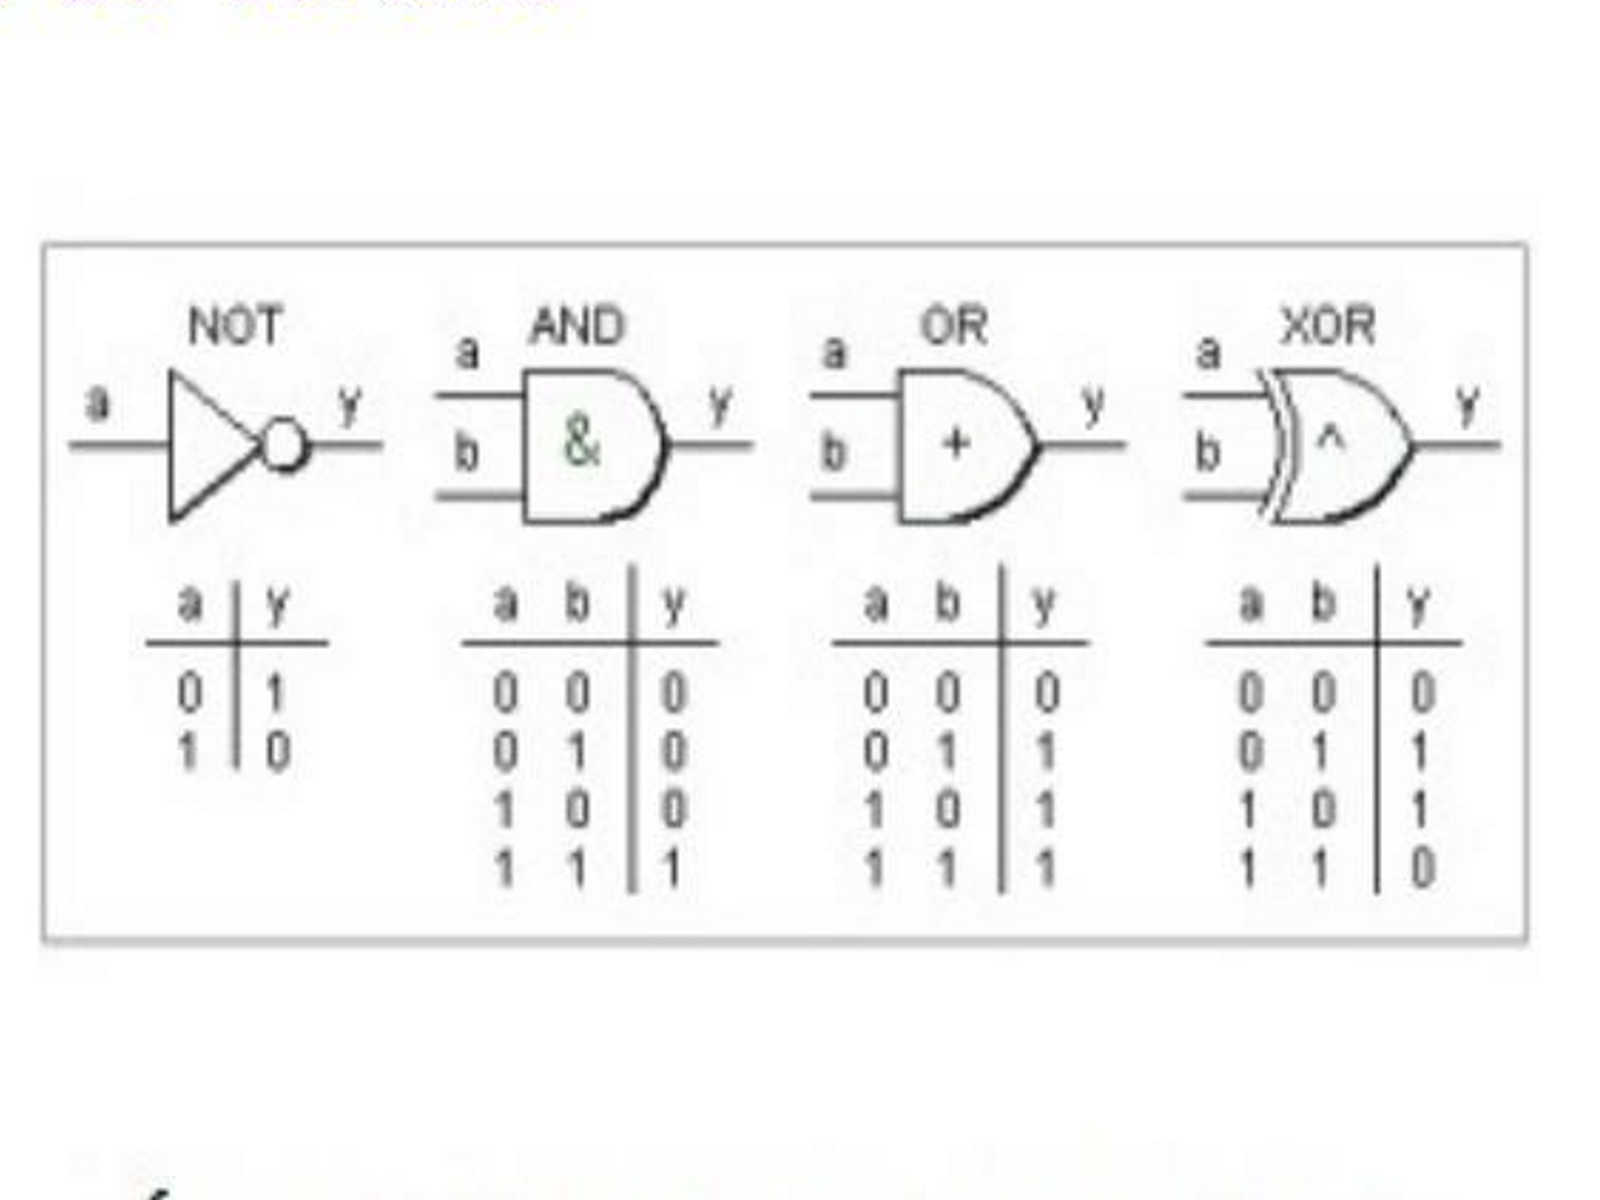
\includegraphics[width=1\linewidth]{figures/ejeSum3.png}
\caption{Algunas compuertas lógicas}
\label{ejeSum3}
\end{figure}
\vspace{0.2cm}
\end{multicols}
\end{example}

\section{Álgebra de Boole Postulados}

En la Figura \ref{proBoo} se muestran los postulados de Boole. 

\begin{figure}[H]
\centering
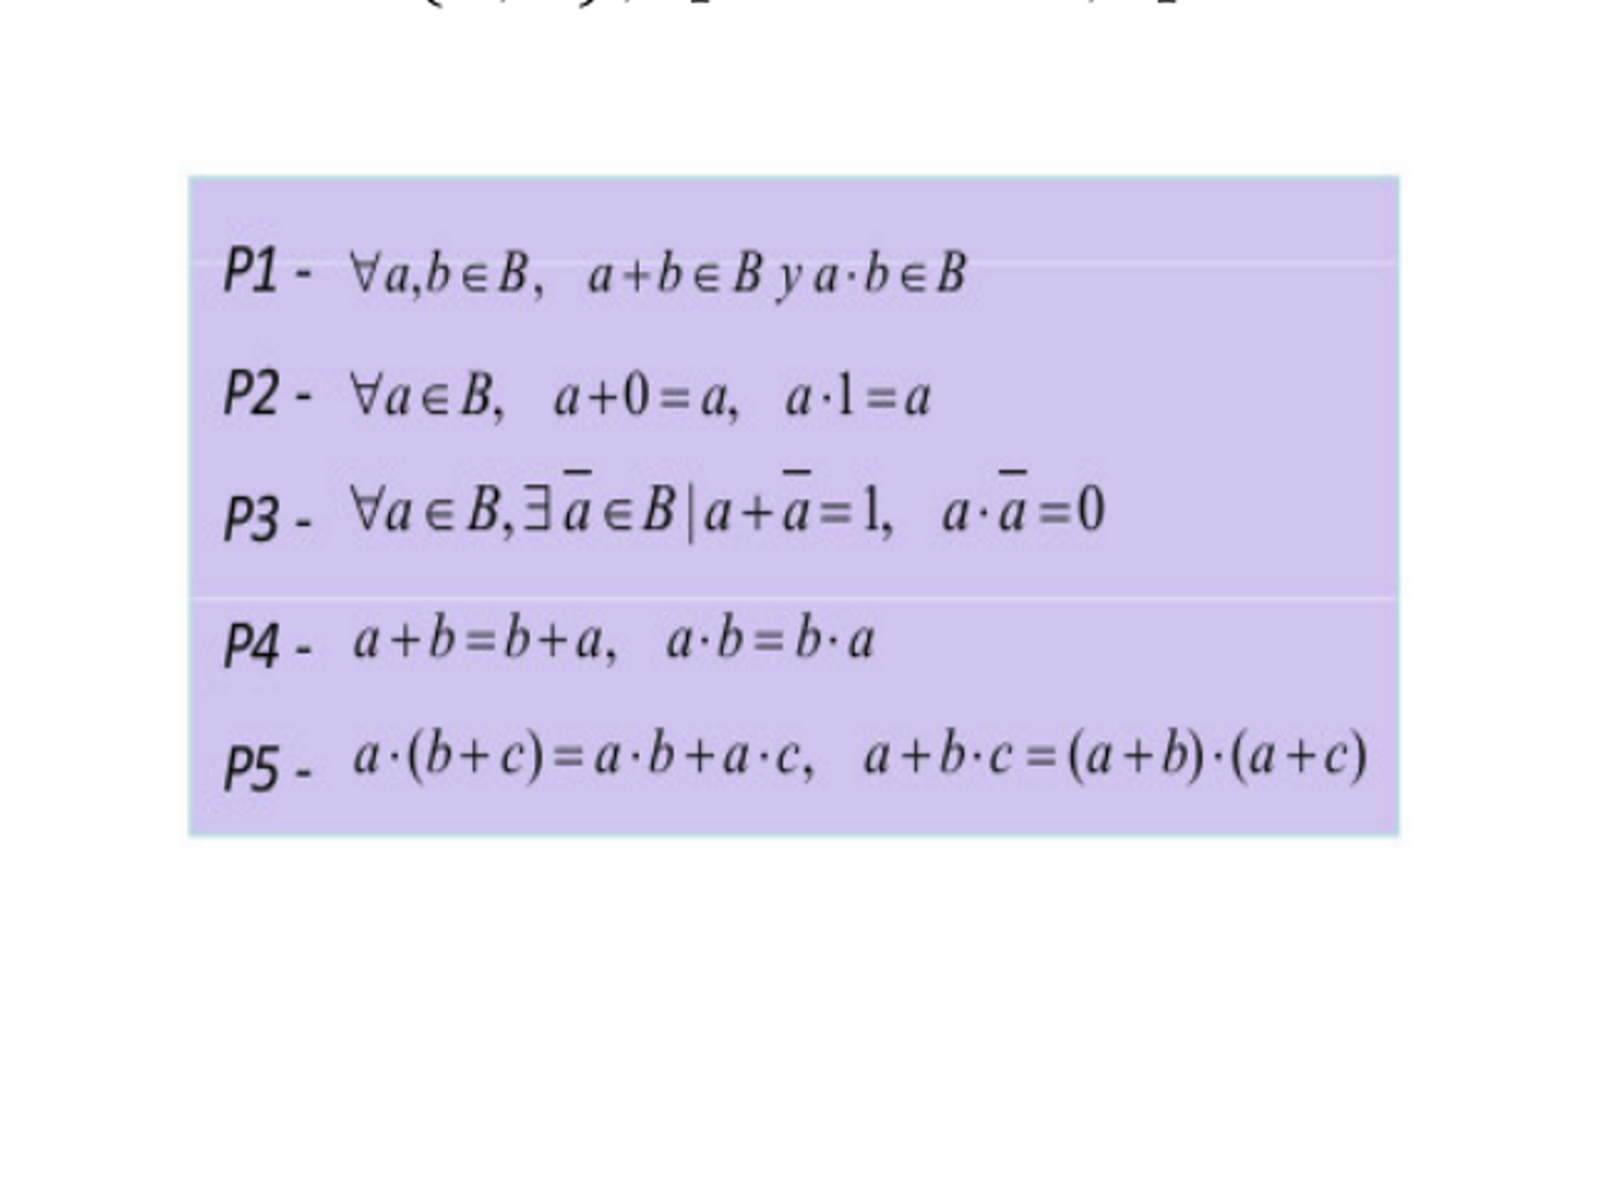
\includegraphics[width=1\linewidth]{figures/proBoo.png}
\caption{Postulados de Boole}
\label{proBoo}
\end{figure}
\vspace{0.2cm}

\chapter{Semana 4}
La Figura \ref{p1} representa algunos símbolos con sus compuertas lógicas equivalentes. Lo que quiere decir cuando si z=a si c=1, es que deja para pasar la señal de entrada. Por otra parte, Z=HI(Hight Impedance) si c=0 es equivalente a decir que la señal no pasa. En pocas palabras, es un interruptor programable.

\begin{figure}[H]
\centering
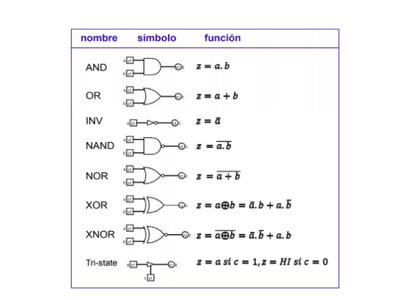
\includegraphics[width=1\linewidth]{figures/p1.png}
\caption{Compuestas lógicas equivalentes}
\label{p1}
\end{figure}
\vspace{0.2cm}

\section{Comparador de un bit}



\begin{multicols}{2}

En la Figura \ref{p2} se muestra el planteamiento para realizar el diseño del comparador de una cadena de bits a partir de un comparador de un bit. Si X>Y se le asigna el valor de 1 a  G, en caso contrario se le asigna 1 a L, si ninguna se cumple, E=1 lo que significa que son iguales. 


\begin{figure}[H]
\centering
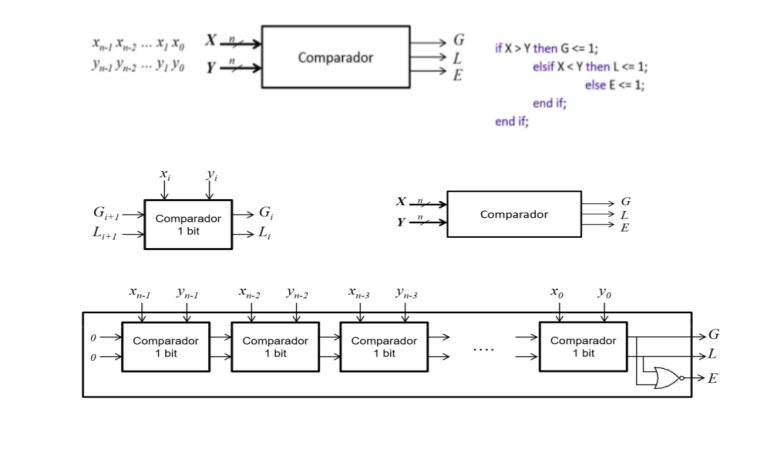
\includegraphics[width=1\linewidth]{figures/p2.png}
\caption{}
\label{p2}
\end{figure}
\vspace{0.2cm}

La lógica para programar es que se va a comenzar a comparar la cadena de bits de la posición más significativa a la menos significativa. Si se sabe que en algún punto que $X>Y$ o viceversa, el código realizaría su función hasta ese punto. Si por ejemplo en sistema decimal se sabe que dos números pueden tener unidades de mil y si en uno de ellos es mayor en las unidades de mil el otro va a ser menor sin importar cuales sean sus dígitos en las demás unidades. En la Figura \ref{p3} se representa esta lógica. 

\begin{figure}[H]
\centering
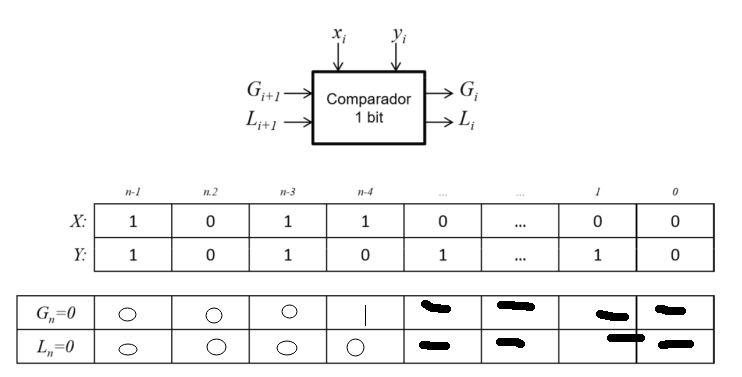
\includegraphics[width=1\linewidth]{figures/p3.png}
\caption{Lógica del comparador de un bit}
\label{p3}
\end{figure}
\vspace{0.2cm}

La Figura \ref{p4}  muestra  una tabla con los valores con todos los posibles valores que se pueden obtener según las cuatro entradas. Se tienen cuatro entradas, porque se está pensando en un proceso en el cual, se vuelva a utilizar reiterativamente un bloque. La \textbf{x} en la tabla significa que los valores que tome no son relevantes.

\begin{figure}[H]
\centering
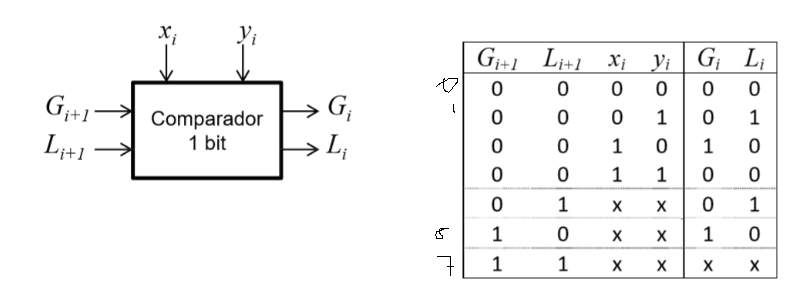
\includegraphics[width=1\linewidth]{figures/p4.png}
\caption{Tablas de valores}
\label{p4}
\end{figure}
\vspace{0.2cm}
 
Actividad\\
Deduzca la ecuación boleana de la Figura \ref{p4}\\
\textcolor{red}{Mi análisis}\\

$G_i= \overline{G}\cdot \overline{L}\cdot x \cdot \overline{y} + G \cdot \overline{L}\cdot \overline{x}  \cdot \overline{y}+G\cdot \overline{L}\cdot x  \cdot \overline{y}  +G\cdot \overline{L}\cdot \overline{x}  \cdot y + G\cdot \overline{L}\cdot x  \cdot y + G\cdot L\cdot \overline{x}  \cdot y + G \cdot L \cdot x \cdot y$\\


\textcolor{red}{Análisis del docente}

Se obtiene directamente de la tabla que:

$Gi=\overline{G}\cdot \overline{L}\cdot x \cdot \overline{y} + G \cdot \overline{L}$

Para simplificar términos se puede elegir un par de ecuaciones de la fila \textcolor{blue}{6} y \textcolor{green}{7} y quedaría de la siguiente manera:\\
 
$Gi=\overline{G}\cdot \overline{L}\cdot x \cdot \overline{y} + \textcolor{blue}{G\cdot \overline{L}\cdot x \cdot \overline{y}} + G \cdot \overline{L}+\textcolor{green}{G \cdot L}$\\


Al utilizar propiedades se obtiene:\\


$Gi=\overline{L}\cdot x \cdot \overline{y}\cdot (\overline{G} + \textcolor{blue}{G}) + G \cdot( \overline{L}+\textcolor{green}{L})$\\


Para finalizar se obtiene:\\


$Gi=\overline{L_{i+1}}\cdot x \cdot \overline{y} + G_{i+1}$\footnote{el i+1 significa que está atrasado}\\



Para el caso de encontrar una función booleana, se procede de manera similar y se obtiene:\\

$L_i=G_{i+1} \cdot \overline{x} \cdot y+L_{i+1}$

\end{multicols}

\section{Mapas de Karnaugh}

\begin{multicols}{2}
Ahora, suponga que la reducción de los mintérminos se hace más compleja, tal como se presenta en la en el comparador de 2 bits que se ilustra en la Figura \ref{p5}.

\begin{figure}[H]
\centering
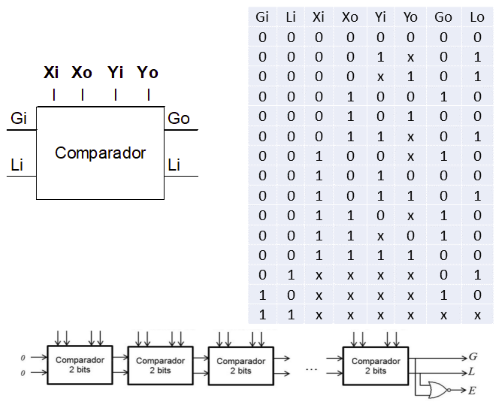
\includegraphics[width=1\linewidth]{figures/p5.png}
\caption{}
\label{p5}
\end{figure}
\vspace{0.2cm}

Se intercepta tanto fila como columna y se obtiene un mapa de Karnaugh como se ilustra en la Figura \ref{k1} 

\begin{figure}[H]
\centering
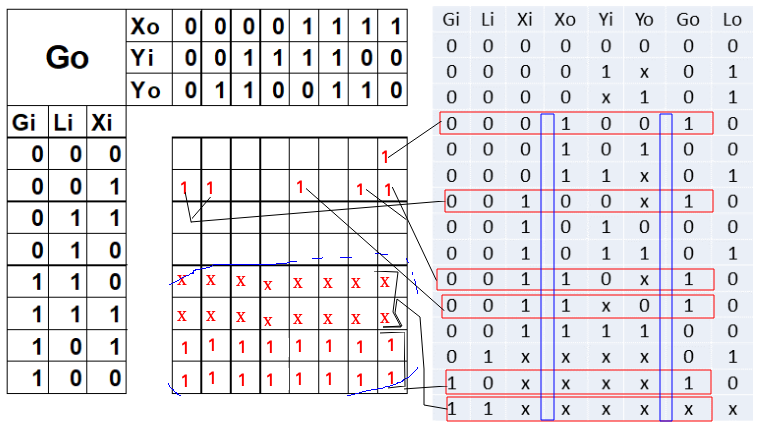
\includegraphics[width=1\linewidth]{figures/k1.png}
\caption{Mapa de Karnaugh}
\label{k1}
\end{figure}
\vspace{0.2cm}
Ahora se procede a hallar simetrías, la primera ecuación que se observa es: $\textcolor{blue}{f_1=Gi}$ ya que el único que no varía. 

\begin{figure}[H]
\centering
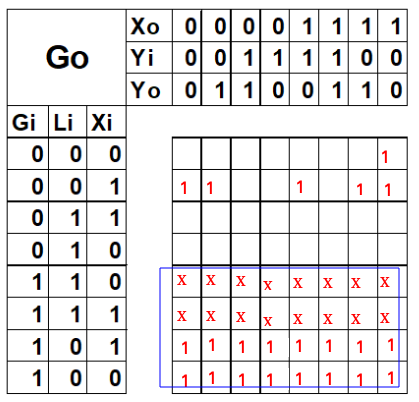
\includegraphics[width=1\linewidth]{figures/k2.png}
\caption{Simetrías}
\label{k2}
\end{figure}
\vspace{0.2cm}

El próximo es: $\textcolor{blue}{f_2=\overline{L_i} \cdot X_i \cdot \overline{Y_i}}$ ya que los demás cambian de valor y eso los hace irrelevantes. 

\begin{figure}[H]
\centering
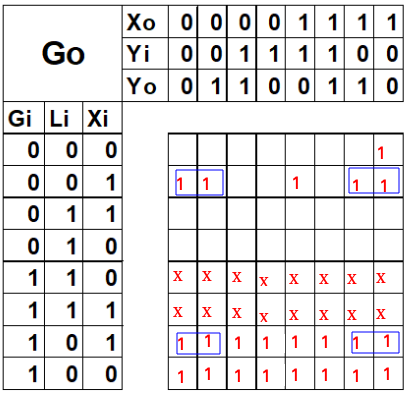
\includegraphics[width=1\linewidth]{figures/k3.png}
\caption{}
\label{}
\end{figure}
\vspace{0.2cm}

$f_3=\textcolor{blue}{\overline{L_i} \cdot X_i \cdot X_0\cdot y_i \cdot \overline{y_o}}$
]
\begin{figure}[H]
\centering
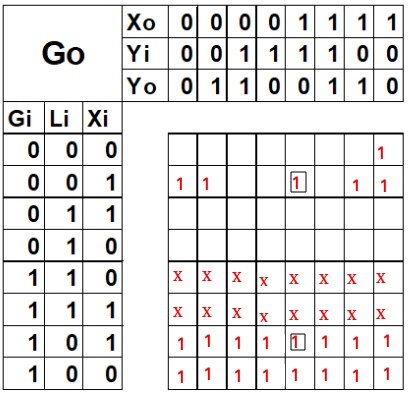
\includegraphics[width=1\linewidth]{figures/k4.png}
\caption{}
\label{k4}
\end{figure}
\vspace{0.2cm}


$f_4=\textcolor{blue}{\overline{L_i} \cdot \overline{X_i} \cdot X_0\cdot \overline{y_i}  \cdot \overline{y_o}}$

\begin{figure}[H]
\centering
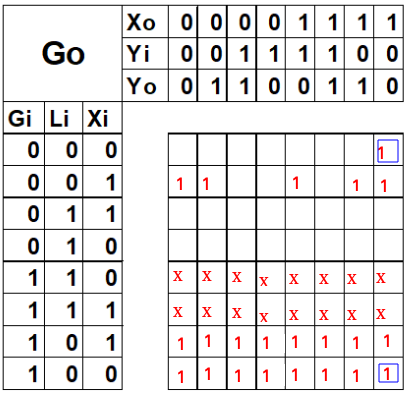
\includegraphics[width=1\linewidth]{figures/k5.png}
\caption{}
\label{k5}
\end{figure}
\vspace{0.2cm}

Al resumir todas las respuestas se tiene:

$\textcolor{blue}{G_0=Gi + \overline{L_i} \cdot X_i \cdot \overline{Y_i} + \overline{L_i} \cdot X_i \cdot X_0\cdot y_i \cdot \overline{y_o}}+ 
 \textcolor{blue}{\overline{L_i} \cdot \overline{ X_i} \cdot X_0 \cdot \overline{y_i}  \cdot \overline{y_o}}$

Ahora se van a analizar las respuestas para L, la Figura \ref{k6} representa el mapa de Karnaugh 

\begin{figure}[H]
\centering
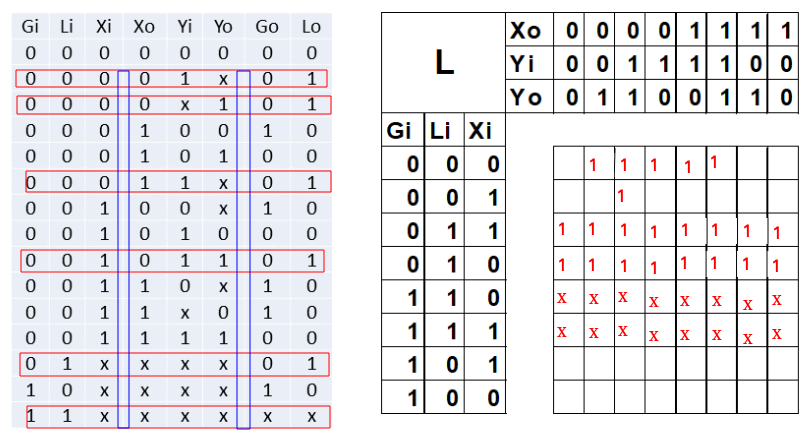
\includegraphics[width=1\linewidth]{figures/k6.png}
\caption{}
\label{k6}
\end{figure}
\vspace{0.2cm}

Paso a seguir es plantear las ecuaciones booleanas.\\
$l_1=\textcolor{blue}{L_i}$

\begin{figure}[H]
\centering
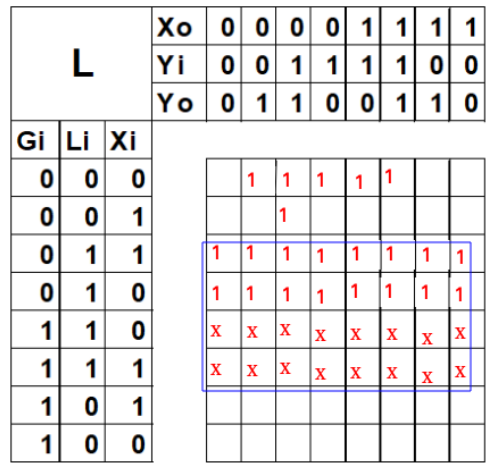
\includegraphics[width=1\linewidth]{figures/k7.png}
\caption{}
\label{k7}
\end{figure}
\vspace{0.2cm}


$l_2=\textcolor{blue}{\overline{G_i} \cdot \overline{X_i} \cdot Y_i}$

\begin{figure}[H]
\centering
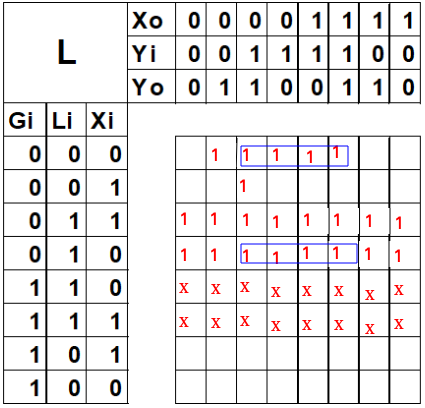
\includegraphics[width=1\linewidth]{figures/k8.png}
\caption{}
\label{k8}
\end{figure}
\vspace{0.2cm}

$l_3=\textcolor{blue}{ \overline{G_i} \cdot X_i \cdot \overline{X_0} \cdot Y_i \cdot Y_o}$

\begin{figure}[H]
\centering
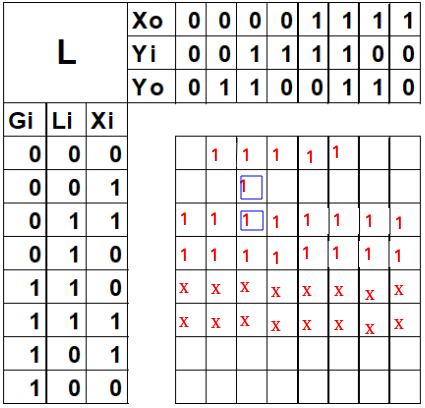
\includegraphics[width=1\linewidth]{figures/k9.png}
\caption{}
\label{k9}
\end{figure}
\vspace{0.2cm}

$l4=\textcolor{blue}{\overline{G_i} \cdot \overline{ X_i} \cdot \overline{X_0} \cdot \overline{Y_i}  \cdot Y_o}$
\begin{figure}[H]
\centering
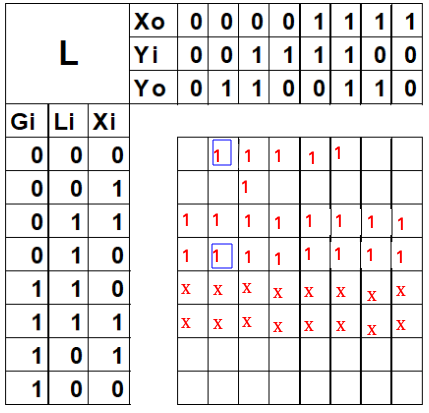
\includegraphics[width=1\linewidth]{figures/k10.png}
\caption{}
\label{k10}
\end{figure}
\vspace{0.2cm}

En resumen se tiene que:\\
$\textcolor{blue}{L_0=L_i+\overline{G_i} \cdot \overline{X_i} \cdot Y_i+\overline{G_i} \cdot X_i \cdot \overline{X_0} \cdot Y_i \cdot Y_o }+\textcolor{blue}{\overline{G_i} \cdot \overline{ X_i} \cdot \overline{X_0} \cdot \overline{Y_i}  \cdot Y_o}$

\end{multicols}

\chapter{Investigaciones}


\chapter{Programación}

\begin{figure}[H] 
\centering
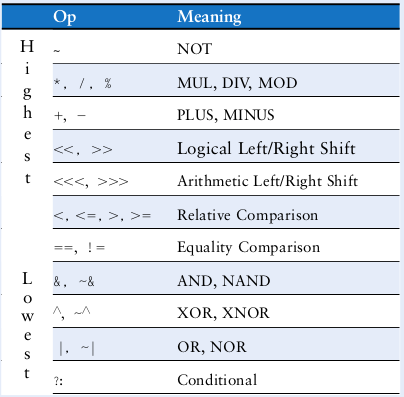
\includegraphics[width=1\linewidth]{figures/a1.png}
\caption{Precedencia entre operadores\cite[Pág . ?]{Harris}}
\label{a1}
\end{figure}
\vspace{0.2cm}

\section{Retraso}

La función booleana $y=\overline{a}\overline{b}\textbf{c}+a\overline{b}\textbf{c}+a\overline{b}c$ puede ser programada en Verilog como sigue \cite[Pág. 183]{Harris}

\begin{lstlisting}[frame=single]
'timescale 1ns/1ps  #' timescale unit/precision.  

module example (a,b,c,y)
input a;
input b;
input c;
output y;

wire ab, bb, cb, n1, n2, n3;

assign #1 {ab,bb,cb}= ~ {a,b,c};
assign #2  n1= ab & bb & cb;
assign #2  n2= a & bb & cb;
assign #2  n3= a & bb & c;
assign #4 y=n1 | n2 | n3;

endmodule

\end{lstlisting}

Es buena idea programar en módulos para evitar mezclar la descripción funcional y estructural. Al instanciar varios módulos se puede describir de manera funcional e individualmente se hace de manera estructural. 


\section{Lógica secuencial}
\subsection{registros}

\textit{always}: Guarda el último evento hasta que otro lo cambie explicitamente.


\chapter{Videos complementarios}
%\href{run:./a.pdf}{Imagen a}

\href{https://www.youtube.com/watch?v=ypz23yWrwf0&feature=youtu.be}{Clases taller 2020\_ 03\_ 23-27 }\\











\bibliography{myBooks}
\bibliographystyle{unsrt} 


\end{document}



   


% Some examples to inset figures
%
%\begin{figure}[H]
%\centering
%\includegraphics[width=1\linewidth]{figures/z_propertiesUnilateral1.png}
%\caption{z-properties unilateral.}
%\label{z_propertiesUnilateral1}
%\end{figure}
